\documentclass[11pt]{report}
\usepackage{./assignment}
\usepackage{slashbox}
%\usepackage{enumitem}
%\usepackage{stmaryrd}
%\usepackage{cprotect}
\usepackage{graphicx}
\usepackage{subfigure}
\renewcommand{\bibname}{References}

\RequirePackage{latexsym}
\RequirePackage{amsmath}
\RequirePackage{amssymb}
\RequirePackage{bm}
\RequirePackage{url}
\RequirePackage{algorithmic}
\RequirePackage{algorithm2e}


%%%%%%%% Stock standard definitions %%%%%%%%%%%%%%%

%\newcommand{\ab}{\mathbf{a}}
%\newcommand{\bb}{\mathbf{b}}
%\newcommand{\cbb}{\mathbf{c}}
%\newcommand{\db}{\mathbf{d}}
%\newcommand{\eb}{\mathbf{e}}
%\newcommand{\fb}{\mathbf{f}}
%\newcommand{\gb}{\mathbf{g}}
%\newcommand{\hb}{\mathbf{h}}
%\newcommand{\ib}{\mathbf{i}}
%\newcommand{\jb}{\mathbf{j}}
%\newcommand{\kb}{\mathbf{k}}
%\newcommand{\lb}{\mathbf{l}}
%\newcommand{\mb}{\mathbf{m}}
%\newcommand{\nbb}{\mathbf{n}}
%\newcommand{\ob}{\mathbf{o}}
%\newcommand{\pb}{\mathbf{p}}
%\newcommand{\qb}{\mathbf{q}}
%\newcommand{\rb}{\mathbf{r}}
%\newcommand{\sbb}{\mathbf{s}}
%\newcommand{\tb}{\mathbf{t}}
%\newcommand{\ub}{\mathbf{u}}
%\newcommand{\vb}{\mathbf{v}}
%\newcommand{\wb}{\mathbf{w}}
%\newcommand{\xb}{\mathbf{x}}
%\newcommand{\yb}{\mathbf{y}}
%\newcommand{\zb}{\mathbf{z}}
%
%\newcommand{\abtil}{\tilde{\ab}}
%\newcommand{\bbtil}{\tilde{\bb}}
%\newcommand{\cbtil}{\tilde{\cbb}}
%\newcommand{\dbtil}{\tilde{\db}}
%\newcommand{\ebtil}{\tilde{\eb}}
%\newcommand{\fbtil}{\tilde{\fb}}
%\newcommand{\gbtil}{\tilde{\gb}}
%\newcommand{\hbtil}{\tilde{\hb}}
%\newcommand{\ibtil}{\tilde{\ib}}
%\newcommand{\jbtil}{\tilde{\jb}}
%\newcommand{\kbtil}{\tilde{\kb}}
%\newcommand{\lbtil}{\tilde{\lb}}
%\newcommand{\mbtil}{\tilde{\mb}}
%\newcommand{\nbtil}{\tilde{\nbb}}
%\newcommand{\obtil}{\tilde{\ob}}
%\newcommand{\pbtil}{\tilde{\pb}}
%\newcommand{\qbtil}{\tilde{\qb}}
%\newcommand{\rbtil}{\tilde{\rb}}
%\newcommand{\sbtil}{\tilde{\sbb}}
%\newcommand{\tbtil}{\tilde{\tb}}
%\newcommand{\ubtil}{\tilde{\ub}}
%\newcommand{\vbtil}{\tilde{\vb}}
%\newcommand{\wbtil}{\tilde{\wb}}
%\newcommand{\xbtil}{\tilde{\xb}}
%\newcommand{\ybtil}{\tilde{\yb}}
%\newcommand{\zbtil}{\tilde{\zb}}
%
%
%\newcommand{\atil}{\tilde{a}}
%\newcommand{\btil}{\tilde{b}}
%\newcommand{\ctil}{\tilde{c}}
%\newcommand{\dtil}{\tilde{d}}
%\newcommand{\etil}{\tilde{e}}
%\newcommand{\ftil}{\tilde{f}}
%\newcommand{\gtil}{\tilde{g}}
%\newcommand{\htil}{\tilde{h}}
%\newcommand{\itil}{\tilde{i}}
%\newcommand{\jtil}{\tilde{j}}
%\newcommand{\ktil}{\tilde{k}}
%\newcommand{\ltil}{\tilde{l}}
%\newcommand{\mtil}{\tilde{m}}
%\newcommand{\ntil}{\tilde{n}}
%\newcommand{\otil}{\tilde{o}}
%\newcommand{\ptil}{\tilde{p}}
%\newcommand{\qtil}{\tilde{q}}
%\newcommand{\rtil}{\tilde{r}}
%\newcommand{\stil}{\tilde{s}}
%\newcommand{\ttil}{\tilde{t}}
%\newcommand{\util}{\tilde{u}}
%\newcommand{\vtil}{\tilde{v}}
%\newcommand{\wtil}{\tilde{w}}
%\newcommand{\xtil}{\tilde{x}}
%\newcommand{\ytil}{\tilde{y}}
%\newcommand{\ztil}{\tilde{z}}
%
%\newcommand{\Atil}{\tilde{A}}
%\newcommand{\Btil}{\tilde{B}}
%\newcommand{\Ctil}{\tilde{C}}
%\newcommand{\Dtil}{\tilde{D}}
%\newcommand{\Etil}{\tilde{E}}
%\newcommand{\Ftil}{\tilde{F}}
%\newcommand{\Gtil}{\tilde{G}}
%\newcommand{\Htil}{\tilde{H}}
%\newcommand{\Itil}{\tilde{I}}
%\newcommand{\Jtil}{\tilde{J}}
%\newcommand{\Ktil}{\tilde{K}}
%\newcommand{\Ltil}{\tilde{L}}
%\newcommand{\Mtil}{\tilde{M}}
%\newcommand{\Ntil}{\tilde{N}}
%\newcommand{\Otil}{\tilde{O}}
%\newcommand{\Ptil}{\tilde{P}}
%\newcommand{\Qtil}{\tilde{Q}}
%\newcommand{\Rtil}{\tilde{R}}
%\newcommand{\Stil}{\tilde{S}}
%\newcommand{\Ttil}{\tilde{T}}
%\newcommand{\Util}{\tilde{U}}
%\newcommand{\Vtil}{\tilde{V}}
%\newcommand{\Wtil}{\tilde{W}}
%\newcommand{\Xtil}{\tilde{X}}
%\newcommand{\Ytil}{\tilde{Y}}
%\newcommand{\Ztil}{\tilde{Z}}
%
%\newcommand{\abar}{\bar{a}}
%\newcommand{\bbar}{\bar{b}}
%\newcommand{\cbar}{\bar{c}}
%\newcommand{\dbar}{\bar{d}}
%\newcommand{\ebar}{\bar{e}}
%\newcommand{\fbar}{\bar{f}}
%\newcommand{\gbar}{\bar{g}}
%\newcommand{\hbr}{\bar{h}}
%\newcommand{\ibar}{\bar{i}}
%\newcommand{\jbar}{\bar{j}}
%\newcommand{\kbar}{\bar{k}}
%\newcommand{\lbar}{\bar{l}}
%\newcommand{\mbar}{\bar{m}}
%\newcommand{\nbar}{\bar{n}}
%\newcommand{\obar}{\bar{o}}
%\newcommand{\pbar}{\bar{p}}
%\newcommand{\qbar}{\bar{q}}
%\newcommand{\rbar}{\bar{r}}
%\newcommand{\sbar}{\bar{s}}
%\newcommand{\tbar}{\bar{t}}
%\newcommand{\ubar}{\bar{u}}
%\newcommand{\vbar}{\bar{v}}
%\newcommand{\wbar}{\bar{w}}
%\newcommand{\xbar}{\bar{x}}
%\newcommand{\ybar}{\bar{y}}
%\newcommand{\zbar}{\bar{z}}
%
%\newcommand{\abbar}{\bar{\ab}}
%\newcommand{\bbbar}{\bar{\bb}}
%\newcommand{\cbbar}{\bar{\cb}}
%\newcommand{\dbbar}{\bar{\db}}
%\newcommand{\ebbar}{\bar{\eb}}
%\newcommand{\fbbar}{\bar{\fb}}
%\newcommand{\gbbar}{\bar{\gb}}
%\newcommand{\hbbar}{\bar{\hb}}
%\newcommand{\ibbar}{\bar{\ib}}
%\newcommand{\jbbar}{\bar{\jb}}
%\newcommand{\kbbar}{\bar{\kb}}
%\newcommand{\lbbar}{\bar{\lb}}
%\newcommand{\mbbar}{\bar{\mb}}
%\newcommand{\nbbar}{\bar{\nbb}}
%\newcommand{\obbar}{\bar{\ob}}
%\newcommand{\pbbar}{\bar{\pb}}
%\newcommand{\qbbar}{\bar{\qb}}
%\newcommand{\rbbar}{\bar{\rb}}
%\newcommand{\sbbar}{\bar{\sbb}}
%\newcommand{\tbbar}{\bar{\tb}}
%\newcommand{\ubbar}{\bar{\ub}}
%\newcommand{\vbbar}{\bar{\vb}}
%\newcommand{\wbbar}{\bar{\wb}}
%\newcommand{\xbbar}{\bar{\xb}}
%\newcommand{\ybbar}{\bar{\yb}}
%\newcommand{\zbbar}{\bar{\zb}}
%
%\newcommand{\Ab}{\mathbf{A}}
%\newcommand{\Bb}{\mathbf{B}}
%\newcommand{\Cb}{\mathbf{C}}
%\newcommand{\Db}{\mathbf{D}}
%\newcommand{\Eb}{\mathbf{E}}
%\newcommand{\Fb}{\mathbf{F}}
%\newcommand{\Gb}{\mathbf{G}}
%\newcommand{\Hb}{\mathbf{H}}
%\newcommand{\Ib}{\mathbf{I}}
%\newcommand{\Jb}{\mathbf{J}}
%\newcommand{\Kb}{\mathbf{K}}
%\newcommand{\Lb}{\mathbf{L}}
%\newcommand{\Mb}{\mathbf{M}}
%\newcommand{\Nb}{\mathbf{N}}
%\newcommand{\Ob}{\mathbf{O}}
%\newcommand{\Pb}{\mathbf{P}}
%\newcommand{\Qb}{\mathbf{Q}}
%\newcommand{\Rb}{\mathbf{R}}
%\newcommand{\Sbb}{\mathbf{S}}
%\newcommand{\Tb}{\mathbf{T}}
%\newcommand{\Ub}{\mathbf{U}}
%\newcommand{\Vb}{\mathbf{V}}
%\newcommand{\Wb}{\mathbf{W}}
%\newcommand{\Xb}{\mathbf{X}}
%\newcommand{\Yb}{\mathbf{Y}}
%\newcommand{\Zb}{\mathbf{Z}}
%
%\newcommand{\Abtil}{\tilde{\Ab}}
%\newcommand{\Bbtil}{\tilde{\Bb}}
%\newcommand{\Cbtil}{\tilde{\Cb}}
%\newcommand{\Dbtil}{\tilde{\Db}}
%\newcommand{\Ebtil}{\tilde{\Eb}}
%\newcommand{\Fbtil}{\tilde{\Fb}}
%\newcommand{\Gbtil}{\tilde{\Gb}}
%\newcommand{\Hbtil}{\tilde{\Hb}}
%\newcommand{\Ibtil}{\tilde{\Ib}}
%\newcommand{\Jbtil}{\tilde{\Jb}}
%\newcommand{\Kbtil}{\tilde{\Kb}}
%\newcommand{\Lbtil}{\tilde{\Lb}}
%\newcommand{\Mbtil}{\tilde{\Mb}}
%\newcommand{\Nbtil}{\tilde{\Nb}}
%\newcommand{\Obtil}{\tilde{\Ob}}
%\newcommand{\Pbtil}{\tilde{\Pb}}
%\newcommand{\Qbtil}{\tilde{\Qb}}
%\newcommand{\Rbtil}{\tilde{\Rb}}
%\newcommand{\Sbtil}{\tilde{\Sbb}}
%\newcommand{\Tbtil}{\tilde{\Tb}}
%\newcommand{\Ubtil}{\tilde{\Ub}}
%\newcommand{\Vbtil}{\tilde{\Vb}}
%\newcommand{\Wbtil}{\tilde{\Wb}}
%\newcommand{\Xbtil}{\tilde{\Xb}}
%\newcommand{\Ybtil}{\tilde{\Yb}}
%\newcommand{\Zbtil}{\tilde{\Zb}}
%
%\newcommand{\Abar}{\bar{A}}
%\newcommand{\Bbar}{\bar{B}}
%\newcommand{\Cbar}{\bar{C}}
%\newcommand{\Dbar}{\bar{D}}
%\newcommand{\Ebar}{\bar{E}}
%\newcommand{\Fbar}{\bar{F}}
%\newcommand{\Gbar}{\bar{G}}
%\newcommand{\Hbar}{\bar{H}}
%\newcommand{\Ibar}{\bar{I}}
%\newcommand{\Jbar}{\bar{J}}
%\newcommand{\Kbar}{\bar{K}}
%\newcommand{\Lbar}{\bar{L}}
%\newcommand{\Mbar}{\bar{M}}
%\newcommand{\Nbar}{\bar{N}}
%\newcommand{\Obar}{\bar{O}}
%\newcommand{\Pbar}{\bar{P}}
%\newcommand{\Qbar}{\bar{Q}}
%\newcommand{\Rbar}{\bar{R}}
%\newcommand{\Sbar}{\bar{S}}
%\newcommand{\Tbar}{\bar{T}}
%\newcommand{\Ubar}{\bar{U}}
%\newcommand{\Vbar}{\bar{V}}
%\newcommand{\Wbar}{\bar{W}}
%\newcommand{\Xbar}{\bar{X}}
%\newcommand{\Ybar}{\bar{Y}}
%\newcommand{\Zbar}{\bar{Z}}
%
%\newcommand{\Abbar}{\bar{\Ab}}
%\newcommand{\Bbbar}{\bar{\Bb}}
%\newcommand{\Cbbar}{\bar{\Cb}}
%\newcommand{\Dbbar}{\bar{\Db}}
%\newcommand{\Ebbar}{\bar{\Eb}}
%\newcommand{\Fbbar}{\bar{\Fb}}
%\newcommand{\Gbbar}{\bar{\Gb}}
%\newcommand{\Hbbar}{\bar{\Hb}}
%\newcommand{\Ibbar}{\bar{\Ib}}
%\newcommand{\Jbbar}{\bar{\Jb}}
%\newcommand{\Kbbar}{\bar{\Kb}}
%\newcommand{\Lbbar}{\bar{\Lb}}
%\newcommand{\Mbbar}{\bar{\Mb}}
%\newcommand{\Nbbar}{\bar{\Nb}}
%\newcommand{\Obbar}{\bar{\Ob}}
%\newcommand{\Pbbar}{\bar{\Pb}}
%\newcommand{\Qbbar}{\bar{\Qb}}
%\newcommand{\Rbbar}{\bar{\Rb}}
%\newcommand{\Sbbar}{\bar{\Sb}}
%\newcommand{\Tbbar}{\bar{\Tb}}
%\newcommand{\Ubbar}{\bar{\Ub}}
%\newcommand{\Vbbar}{\bar{\Vb}}
%\newcommand{\Wbbar}{\bar{\Wb}}
%\newcommand{\Xbbar}{\bar{\Xb}}
%\newcommand{\Ybbar}{\bar{\Yb}}
%\newcommand{\Zbbar}{\bar{\Zb}}
%
%\newcommand{\Ahat}{\hat{A}}
%\newcommand{\Bhat}{\hat{B}}
%\newcommand{\Chat}{\hat{C}}
%\newcommand{\Dhat}{\hat{D}}
%\newcommand{\Ehat}{\hat{E}}
%\newcommand{\Fhat}{\hat{F}}
%\newcommand{\Ghat}{\hat{G}}
%\newcommand{\Hhat}{\hat{H}}
%\newcommand{\Ihat}{\hat{I}}
%\newcommand{\Jhat}{\hat{J}}
%\newcommand{\Khat}{\hat{K}}
%\newcommand{\Lhat}{\hat{L}}
%\newcommand{\Mhat}{\hat{M}}
%\newcommand{\Nhat}{\hat{N}}
%\newcommand{\Ohat}{\hat{O}}
%\newcommand{\Phat}{\hat{P}}
%\newcommand{\Qhat}{\hat{Q}}
%\newcommand{\Rhat}{\hat{R}}
%\newcommand{\Shat}{\hat{S}}
%\newcommand{\That}{\hat{T}}
%\newcommand{\Uhat}{\hat{U}}
%\newcommand{\Vhat}{\hat{V}}
%\newcommand{\What}{\hat{W}}
%\newcommand{\Xhat}{\hat{X}}
%\newcommand{\Yhat}{\hat{Y}}
%\newcommand{\Zhat}{\hat{Z}}
%
%\newcommand{\Abhat}{\hat{\Ab}}
%\newcommand{\Bbhat}{\hat{\Bb}}
%\newcommand{\Cbhat}{\hat{\Cb}}
%\newcommand{\Dbhat}{\hat{\Db}}
%\newcommand{\Ebhat}{\hat{\Eb}}
%\newcommand{\Fbhat}{\hat{\Fb}}
%\newcommand{\Gbhat}{\hat{\Gb}}
%\newcommand{\Hbhat}{\hat{\Hb}}
%\newcommand{\Ibhat}{\hat{\Ib}}
%\newcommand{\Jbhat}{\hat{\Jb}}
%\newcommand{\Kbhat}{\hat{\Kb}}
%\newcommand{\Lbhat}{\hat{\Lb}}
%\newcommand{\Mbhat}{\hat{\Mb}}
%\newcommand{\Nbhat}{\hat{\Nb}}
%\newcommand{\Obhat}{\hat{\Ob}}
%\newcommand{\Pbhat}{\hat{\Pb}}
%\newcommand{\Qbhat}{\hat{\Qb}}
%\newcommand{\Rbhat}{\hat{\Rb}}
%\newcommand{\Sbhat}{\hat{\Sb}}
%\newcommand{\Tbhat}{\hat{\Tb}}
%\newcommand{\Ubhat}{\hat{\Ub}}
%\newcommand{\Vbhat}{\hat{\Vb}}
%\newcommand{\Wbhat}{\hat{\Wb}}
%\newcommand{\Xbhat}{\hat{\Xb}}
%\newcommand{\Ybhat}{\hat{\Yb}}
%\newcommand{\Zbhat}{\hat{\Zb}}
%
%\newcommand{\Acal}{\mathcal{A}}
%\newcommand{\Bcal}{\mathcal{B}}
%\newcommand{\Ccal}{\mathcal{C}}
%\newcommand{\Dcal}{\mathcal{D}}
%\newcommand{\Ecal}{\mathcal{E}}
%\newcommand{\Fcal}{\mathcal{F}}
%\newcommand{\Gcal}{\mathcal{G}}
%\newcommand{\Hcal}{\mathcal{H}}
%\newcommand{\Ical}{\mathcal{I}}
%\newcommand{\Jcal}{\mathcal{J}}
%\newcommand{\Kcal}{\mathcal{K}}
%\newcommand{\Lcal}{\mathcal{L}}
%\newcommand{\Mcal}{\mathcal{M}}
%\newcommand{\Ncal}{\mathcal{N}}
%\newcommand{\Ocal}{\mathcal{O}}
%\newcommand{\Pcal}{\mathcal{P}}
%\newcommand{\Qcal}{\mathcal{Q}}
%\newcommand{\Rcal}{\mathcal{R}}
%\newcommand{\Scal}{{\mathcal{S}}}
%\newcommand{\Tcal}{{\mathcal{T}}}
%\newcommand{\Ucal}{\mathcal{U}}
%\newcommand{\Vcal}{\mathcal{V}}
%\newcommand{\Wcal}{\mathcal{W}}
%\newcommand{\Xcal}{\mathcal{X}}
%\newcommand{\Ycal}{\mathcal{Y}}
%\newcommand{\Zcal}{\mathcal{Z}}
%
%\newcommand{\Atilde}{\widetilde{A}}
%\newcommand{\Btilde}{\widetilde{B}}
%\newcommand{\Ctilde}{\widetilde{C}}
%\newcommand{\Dtilde}{\widetilde{D}}
%\newcommand{\Etilde}{\widetilde{E}}
%\newcommand{\Ftilde}{\widetilde{F}}
%\newcommand{\Gtilde}{\widetilde{G}}
%\newcommand{\Htilde}{\widetilde{H}}
%\newcommand{\Itilde}{\widetilde{I}}
%\newcommand{\Jtilde}{\widetilde{J}}
%\newcommand{\Ktilde}{\widetilde{K}}
%\newcommand{\Ltilde}{\widetilde{L}}
%\newcommand{\Mtilde}{\widetilde{M}}
%\newcommand{\Ntilde}{\widetilde{N}}
%\newcommand{\Otilde}{\widetilde{O}}
%\newcommand{\Ptilde}{\widetilde{P}}
%\newcommand{\Qtilde}{\widetilde{Q}}
%\newcommand{\Rtilde}{\widetilde{R}}
%\newcommand{\Stilde}{\widetilde{S}}
%\newcommand{\Ttilde}{\widetilde{T}}
%\newcommand{\Utilde}{\widetilde{U}}
%\newcommand{\Vtilde}{\widetilde{V}}
%\newcommand{\Wtilde}{\widetilde{W}}
%\newcommand{\Xtilde}{\widetilde{X}}
%\newcommand{\Ytilde}{\widetilde{Y}}
%\newcommand{\Ztilde}{\widetilde{Z}}
%
%
%%%%%%%%% Widely accepted definitions %%%%%%%%%%%%%%%
%
%\newcommand{\CC}{\mathbb{C}} % Complex numbers
%\newcommand{\EE}{\mathbb{E}} % Expectation
%\newcommand{\II}{\mathbb{I}} % Delta Indicator
%\newcommand{\VV}{\mathbb{V}} % Variance
%\newcommand{\KK}{\mathbb{K}} % Arbitrary field
%\newcommand{\MM}{\mathbb{M}} % Median
%\newcommand{\NN}{\mathbb{N}} % Natural numbers
%\newcommand{\PP}{\mathbb{P}} % Probability
%\newcommand{\QQ}{\mathbb{Q}} % Rationals
%\newcommand{\RR}{\mathbb{R}} % Real numbers
%\newcommand{\ZZ}{\mathbb{Z}} % Integers
%\newcommand{\XX}{\mathbb{X}} % Integers
%\newcommand{\YY}{\mathbb{Y}} % Integers
%
%\newcommand{\one}{\mathbf{1}}  % Identity
%\newcommand{\zero}{\mathbf{0}} % Zero
%%\newcommand{\TRUE}{\mathbf{TRUE}}  % True
%%\newcommand{\FALSE}{\mathbf{FALSE}}  % False
%
%\newcommand*{\mini}{\mathop{\mathrm{minimize}}}
%\newcommand*{\maxi}{\mathop{\mathrm{maximize}}}
%\newcommand*{\argmin}{\mathop{\mathrm{argmin}}}
%\newcommand*{\argmax}{\mathop{\mathrm{argmax}}}
%\newcommand{\sgn}{\mathop{\mathrm{sign}}}
%\newcommand{\tr}{\mathop{\mathrm{tr}}}
%\newcommand{\diag}{\mathop{\mathrm{diag}}}
%\newcommand{\rank}{\mathop{\mathrm{rank}}}
%%\newcommand{\ovec}{\mathop{\mathrm{vec}}}
%\newcommand{\traj}{\mathop{\mathrm{Traj}}}
%\newcommand*{\cov}{\mathrm{Cov}}
%\newcommand*{\conv}{\mathrm{conv}}
%\newcommand*{\const}{\mathrm{constant}}
%
%%%%%%%%% Bold Greek Letters %%%%%%%%%%%%%%%
%\newcommand{\sigmab}{\bm{\sigma}}
%\newcommand{\Sigmab}{\mathbf{\Sigma}}
%
%
%%%%%%%%% Mess around with LaTeX %%%%%%%%%%%%%%%
%
%%% Some style files might actually define these variables.
%%% So don't mess with them if they are already defined
%
%\ifx\BlackBox\undefined
%\newcommand{\BlackBox}{\rule{1.5ex}{1.5ex}}  % end of proof
%\fi
%
%\ifx\QED\undefined
%\def\QED{~\rule[-1pt]{5pt}{5pt}\par\medskip}
%\fi
%
%\ifx\proof\undefined
%\newenvironment{proof}{\par\noindent{\bf Proof\ }}{\hfill\BlackBox\\[2mm]}
%%\newenvironment{proof}{\emph{Proof. }}{ \hfill \QED}
%\fi
%
%\ifx\theorem\undefined
%\newtheorem{theorem}{Theorem}
%\newtheorem{example}{Example}
%\newtheorem{property}{Property}
%\newtheorem{lemma}[theorem]{Lemma}
%\newtheorem{proposition}[theorem]{Proposition}
%\newtheorem{remark}[theorem]{Remark}
%\newtheorem{corollary}[theorem]{Corollary}
%\newtheorem{definition}[theorem]{Definition}
%\newtheorem{conjecture}[theorem]{Conjecture}
%\fi
%
%\ifx\axiom\undefined
%\newtheorem{axiom}[theorem]{Axiom}
%\fi
%
%%%%%%%%% Utility functions %%%%%%%%%%%%%%%
%
%\newcommand{\eq}[1]{(\ref{#1})}
%\newcommand{\mymatrix}[2]{\left[\begin{array}{#1} #2 \end{array}\right]}
%\newcommand{\mychoose}[2]{\left(\begin{array}{c} #1 \\ #2 \end{array}\right)}
%\newcommand{\mydet}[1]{\det\left[ #1 \right]}
%\newcommand{\sembrack}[1]{[\![#1]\!]}
%
%\newcommand{\ea}{\emph{et al.}}
%\newcommand{\eg}{\emph{e.g.}}
%\newcommand{\ie}{\emph{i.e.}}
%\newcommand{\iid}{\emph{iid}}
%
%%\newcommand{\alex}[1]{{\bf ALEX: \uppercase{#1}}}
%%\newcommand{\vishy}[1]{{\bf VISHY: \uppercase{#1}}}
%%\newcommand{\rene}[1]{{\bf RENE: \uppercase{#1}}}
%%\newcommand{\karsten}[1]{{\bf KARSTEN: \uppercase{#1}}}
%
%%%%%%%%% Specific symbols for this project %%%%%%%%%%%%%%%
%
%\newcommand{\methodname}{KDE}
%\newcommand{\ind}{\boldsymbol{\mathsf{I}}}
%
%\newcommand{\hsic}{\mathrm{HSIC}}
%\newcommand{\mmd}{\mathrm{MMD}}
%
%%\newcommand{\tDiag}{\textsf{Diag}}
%%\newcommand{\tTr}{\textsf{Tr}}
%%\newcommand{\tE}{\textsf{E}}
%%\newcommand{\tVec}{\textsf{Vec}}
%%\newcommand{\tRank}{\textsf{Rank}}
%
%%%%%%%%%%%%%%%%%%%%%%%%%%%%%%%%%%%%%%%%%%%%%%%%%%%%%%%%%%%%%%%%%%%%%%%%%%%%
%% math symbols and commands
%%%%%%%%%%%%%%%%%%%%%%%%%%%%%%%%%%%%%%%%%%%%%%%%%%%%%%%%%%%%%%%%%%%%%%%%%%%%
%%\newcommand{\eq}[1]{(\ref{#1})}
%%\newcommand{\mymatrix}[2]{\left[\begin{array}{#1} #2 \end{array}\right]}
%
%%brackets
%\newcommand{\inner}[2]{\left\langle #1,#2 \right\rangle}
%\newcommand{\rbr}[1]{\left(#1\right)}
%\newcommand{\sbr}[1]{\left[#1\right]}
%\newcommand{\cbr}[1]{\left\{#1\right\}}
%\newcommand{\nbr}[1]{\left\|#1\right\|}
%\newcommand{\abr}[1]{\left|#1\right|}
%\newcommand{\smallfrac}[2]{{\textstyle \frac{#1}{#2}}}
%\renewcommand{\url}[1]{{\sffamily #1}}
%\newcommand{\arow}[2]{#1_{#2\cdot}}
%\newcommand{\acol}[2]{#1_{\cdot#2}}
%
%\newcommand{\twoco}[1]{\multicolumn{2}{c|}{#1}}
%\def\ci{\perp\!\!\!\perp}
%
%
%%%% Local Variables:
%%%% mode: latex
%%%% TeX-master: "./SIGMOD06/SIGMODB06.tex"
%%%% End:
%
%
%% by xinhua
%\newcommand{\delhat}{\hat{\delta}}
%\newcommand{\delbar}{\bar{\delta}}
%\newcommand{\HH}{\mathbb{H}} % Arbitrary field
%\newcommand{\ve}{\varepsilon}
%\newcommand{\dom}{\mathrm{dom}}
%
%%%% Local Variables:
%%%% mode: latex
%%%% TeX-master: "./SIGMOD06/SIGMODB06.tex"
%%%% End:
%%%%%%%%%%%%%%%%%%%%%%%%%%%%%%%%%%%%%%%%%%%%%%%%%%%%%%%%%%%%%%%%%%%%%%%%%%%
%%                               PROOF, THEOREM, and FRIENDS
%%%%%%%%%%%%%%%%%%%%%%%%%%%%%%%%%%%%%%%%%%%%%%%%%%%%%%%%%%%%%%%%%%%%%%%%%%%%
%
%%\newcommand{\BlackBox}{\rule{1.5ex}{1.5ex}}  % end of proof
%%\newenvironment{proof}{\par\noindent{\bf Proof.\ }}{\hfill\BlackBox\\[2mm]}
%
%%\newcounter{all_counter}
%%\newcounter{lemma_counter}
%%\newcounter{proposition_counter}
%%\newcounter{remark_counter}
%%\newcounter{corollary_counter}
%%\newcounter{definition_counter}
%%\newcounter{conjecture_counter}
%%\newcounter{axiom_counter}
%%
%%\setcounter{lemma_counter}{0} \setcounter{proposition_counter}{0}
%%\setcounter{remark_counter}{0} \setcounter{corollary_counter}{0}
%%\setcounter{definition_counter}{0}
%%\setcounter{conjecture_counter}{0} \setcounter{axiom_counter}{0}
%
%%\newtheorem{lemma}[lemma_counter]{Lemma}
%%\newtheorem{proposition}[proposition_counter]{Proposition}
%%\newtheorem{remark}[remark_counter]{Remark}
%%\newtheorem{corollary}[corollary_counter]{Corollary}
%%\newtheorem{definition}[definition_counter]{Definition}
%%\newtheorem{conjecture}[conjecture_counter]{Conjecture}
%%\newtheorem{axiom}[axiom_counter]{Axiom}
%
%\newtheorem{assumption}[theorem]{Assumption}
%
%\newcommand{\ahat}{\hat{a}}
%\newcommand{\bhat}{\hat{b}}
%\newcommand{\chat}{\hat{c}}
%\newcommand{\dhat}{\hat{d}}
%\newcommand{\ehat}{\hat{e}}
%\newcommand{\fhat}{\hat{f}}
%\newcommand{\ghat}{\hat{g}}
%\newcommand{\hhat}{\hat{h}}
%\newcommand{\ihat}{\hat{i}}
%\newcommand{\jhat}{\hat{j}}
%\newcommand{\khat}{\hat{k}}
%\newcommand{\lhat}{\hat{l}}
%\newcommand{\mhat}{\hat{m}}
%\newcommand{\nhat}{\hat{n}}
%\newcommand{\ohat}{\hat{o}}
%\newcommand{\phat}{\hat{p}}
%\newcommand{\qhat}{\hat{q}}
%\newcommand{\rhat}{\hat{r}}
%\newcommand{\shat}{\hat{s}}
%\newcommand{\that}{\hat{t}}
%\newcommand{\uhat}{\hat{u}}
%\newcommand{\vhat}{\hat{v}}
%\newcommand{\what}{\hat{w}}
%\newcommand{\xhat}{\hat{x}}
%\newcommand{\yhat}{\hat{y}}
%\newcommand{\zhat}{\hat{z}}
%
%\newcommand{\abhat}{\hat{\ab}}
%\newcommand{\bbhat}{\hat{\bb}}
%\newcommand{\cbhat}{\hat{\cb}}
%\newcommand{\dbhat}{\hat{\db}}
%\newcommand{\ebhat}{\hat{\eb}}
%\newcommand{\fbhat}{\hat{\fb}}
%\newcommand{\gbhat}{\hat{\gb}}
%\newcommand{\hbhat}{\hat{\hb}}
%\newcommand{\ibhat}{\hat{\ib}}
%\newcommand{\jbhat}{\hat{\jb}}
%\newcommand{\kbhat}{\hat{\kb}}
%\newcommand{\lbhat}{\hat{\lb}}
%\newcommand{\mbhat}{\hat{\mb}}
%\newcommand{\nbhat}{\hat{\nb}}
%\newcommand{\obhat}{\hat{\ob}}
%\newcommand{\pbhat}{\hat{\pb}}
%\newcommand{\qbhat}{\hat{\qb}}
%\newcommand{\rbhat}{\hat{\rb}}
%\newcommand{\sbhat}{\hat{\sb}}
%\newcommand{\tbhat}{\hat{\tb}}
%\newcommand{\ubhat}{\hat{\ub}}
%\newcommand{\vbhat}{\hat{\vb}}
%\newcommand{\wbhat}{\hat{\wb}}
%\newcommand{\xbhat}{\hat{\xb}}
%\newcommand{\ybhat}{\hat{\yb}}
%\newcommand{\zbhat}{\hat{\zb}}
%
%\renewcommand{\vec}[1]{\mathbf{\boldsymbol{#1}}}
%
%\newcommand{\avec}{\vec{a}}
%\newcommand{\bvec}{\vec{b}}
%\newcommand{\cvec}{\vec{c}}
%\newcommand{\dvec}{\vec{d}}
%\newcommand{\evec}{\vec{e}}
%\newcommand{\fvec}{\vec{f}}
%\newcommand{\gvec}{\vec{g}}
%\newcommand{\hvec}{\vec{h}}
%\newcommand{\ivec}{\vec{i}}
%\newcommand{\jvec}{\vec{j}}
%\newcommand{\kvec}{\vec{k}}
%\newcommand{\lvec}{\vec{l}}
%\newcommand{\mvec}{\vec{m}}
%\newcommand{\nvec}{\vec{n}}
%\newcommand{\ovec}{\vec{o}}
%\newcommand{\pvec}{\vec{p}}
%\newcommand{\qvec}{\vec{q}}
%\newcommand{\rvec}{\vec{r}}
%\newcommand{\svec}{\vec{s}}
%\newcommand{\tvec}{\vec{t}}
%\newcommand{\uvec}{\vec{u}}
%\newcommand{\vvec}{\vec{v}}
%\newcommand{\wvec}{\vec{w}}
%\newcommand{\xvec}{\vec{x}}
%\newcommand{\yvec}{\vec{y}}
%\newcommand{\zvec}{\vec{z}}
%
%\newcommand{\Avec}{\vec{A}}
%\newcommand{\Bvec}{\vec{B}}
%\newcommand{\Cvec}{\vec{C}}
%\newcommand{\Dvec}{\vec{D}}
%\newcommand{\Evec}{\vec{E}}
%\newcommand{\Fvec}{\vec{F}}
%\newcommand{\Gvec}{\vec{G}}
%\newcommand{\Hvec}{\vec{H}}
%\newcommand{\Ivec}{\vec{I}}
%\newcommand{\Jvec}{\vec{J}}
%\newcommand{\Kvec}{\vec{K}}
%\newcommand{\Lvec}{\vec{L}}
%\newcommand{\Mvec}{\vec{M}}
%\newcommand{\Nvec}{\vec{N}}
%\newcommand{\Ovec}{\vec{O}}
%\newcommand{\Pvec}{\vec{P}}
%\newcommand{\Qvec}{\vec{Q}}
%\newcommand{\Rvec}{\vec{R}}
%\newcommand{\Svec}{\vec{S}}
%\newcommand{\Tvec}{\vec{T}}
%\newcommand{\Uvec}{\vec{U}}
%\newcommand{\Vvec}{\vec{V}}
%\newcommand{\Wvec}{\vec{W}}
%\newcommand{\Xvec}{\vec{X}}
%\newcommand{\Yvec}{\vec{Y}}
%\newcommand{\Zvec}{\vec{Z}}
%
%
%\newcommand{\alphavec}{\vec{\alpha}}
%\newcommand{\betavec}{\vec{\beta}}
%\newcommand{\deltavec}{\vec{\delta}}
%\newcommand{\etavec}{\vec{\eta}}
%\newcommand{\phivec}{\vec{\phi}}
%\newcommand{\psivec}{\vec{\psi}}
%\newcommand{\thetavec}{\vec{\theta}}
%\newcommand{\muvec}{\vec{\mu}}
%\newcommand{\xivec}{\vec{\xi}}
%
%
%\newcommand{\alphab}{\boldsymbol{\alpha}}
%\newcommand{\betab}{\boldsymbol{\beta}}
%\newcommand{\gammab}{\boldsymbol{\gamma}}
%\newcommand{\thetab}{\boldsymbol{\theta}}
%\newcommand{\mub}{\boldsymbol{\mu}}
%\newcommand{\xib}{\boldsymbol{\xi}}
%\newcommand{\Deltab}{\boldsymbol{\Delta}}
%\newcommand{\Pib}{\boldsymbol{\Pi}}
%\newcommand{\etab}{\boldsymbol{\eta}}
%\newcommand{\taub}{\boldsymbol{\tau}}
%\newcommand{\lambdab}{\boldsymbol{\lambda}}
%\newcommand{\pitil}{\tilde{\pi}}
%
%\newcommand{\rmd}{\mathrm{d}}
%\newcommand{\HSIC}{\mathrm{HSIC}}
%
%\newcommand{\dir}{\mathrm{Dir}}
%\newcommand{\dirp}{\mathrm{DP}}
%\newcommand{\multi}{\mathrm{Multi}}
%\newcommand{\gam}{\mathrm{Gamma}}
%\newcommand{\var}{\mathrm{Var}}
%\newcommand{\cor}{\mathrm{Corr}}
%\newcommand{\bet}{\mathrm{Beta}}
%
%\newcommand{\ra}{\rightarrow}
%
%\newcommand{\idf}{{\tt idf}}
%
%\newcommand{\tp}{\text{tp}}
%\newcommand{\fn}{\text{fn}}
%\newcommand{\fp}{\text{fp}}
%\newcommand{\tpb}{\overline{\text{tp}}}
%\newcommand{\fnb}{\overline{\text{fn}}}
%\newcommand{\fpb}{\overline{\text{fp}}}
%\newcommand{\pre}{\text{Pre}}
%\newcommand{\rec}{\text{Rec}}
%\newcommand{\fs}{\text{F-score}}
%\newcommand{\opt}{\text{opt}}
%
%\newcommand{\topics}{{\tt topics}}
%\newcommand{\industries}{{\tt industries}}
%\newcommand{\regions}{{\tt regions}}
%\newcommand{\ip}{{\tt ip}}
%\newcommand{\category}{{\tt category}}
%
%\newcommand{\grad}{{\nabla}}
%\newcommand{\gradbar}{{\bar{\nabla}}}
%\newcommand{\mbarr}{{\overline{M(r)}}}
%\newcommand{\card}{{\mathrm{card }}}
%\newcommand{\MED}{{\text{MED}}}
%\newcommand{\mubar}{\bar{\mu}}
%\newcommand{\emp}{{\mathrm{emp}}}
%\newcommand{\core}{{\mathrm{core}}}
%\newcommand{\zerob}{{\mathbf{0}}}
%\newcommand{\co}{{\mathrm{co}}}
%\newcommand{\argsup}{\mathop{\mathrm{argsup}}}
%\newcommand{\intr}{{\mathrm{int}}}
%\newcommand{\bd}{{\mathrm{bd}}}
%\newcommand{\BMRM}{{BMRM}}
%\newcommand{\where}{{\quad \text{where} \quad}}
%\newcommand{\lcg}{{\textit{l.c.g}}}
%\newcommand{\gradtil}{{\tilde{\grad}}}
%\newcommand{\alphabtil}{{\tilde{\alphab}}}
%\newcommand{\gstar}{{g^{\star}}}
%\newcommand{\fstar}{{f^{\star}}}
%
%
%\newcommand{\sqrttwo}{{\sqrt{2}}}
%\newcommand{\invsqrttwo}{{\frac{1}{\sqrt{2}}}}
%\newcommand{\invtwo}{{\frac{1}{2}}}
%\newcommand{\phihat}{{\hat{\phi}}}
%\newcommand{\cp}{\mathrm{cp}}
%\newcommand{\liblinear}{{\sf liblinear}}
%\newcommand{\lsbmrm}{{\sf ls-bmrm}}
%\newcommand{\qpbmrm}{{\sf qp-bmrm}}
%\newcommand{\pegasos}{{\sf pegasos}}
%\newcommand{\pegan}{{\sf pegasos-$n$}}
%\newcommand{\pegaone}{{\sf pegasos-1}}
%\newcommand{\nest}{{\sf Pragam}}
%\newcommand{\nestb}{{\sf Pragam-b}}
%\newcommand{\err}{{\sf err}}



\newcommand{\ab}{\mathbf{a}}
\newcommand{\bb}{\mathbf{b}}
\newcommand{\cbb}{\mathbf{c}}
\newcommand{\db}{\mathbf{d}}
\newcommand{\eb}{\mathbf{e}}
\newcommand{\fb}{\mathbf{f}}
\newcommand{\gb}{\mathbf{g}}
\newcommand{\hb}{\mathbf{h}}
\newcommand{\ib}{\mathbf{i}}
\newcommand{\jb}{\mathbf{j}}
\newcommand{\kb}{\mathbf{k}}
\newcommand{\lb}{\mathbf{l}}
\newcommand{\mb}{\mathbf{m}}
\newcommand{\nbb}{\mathbf{n}}
\newcommand{\ob}{\mathbf{o}}
\newcommand{\pb}{\mathbf{p}}
\newcommand{\qb}{\mathbf{q}}
\newcommand{\rb}{\mathbf{r}}
\newcommand{\sbb}{\mathbf{s}}
\newcommand{\tb}{\mathbf{t}}
\newcommand{\ub}{\mathbf{u}}
\newcommand{\vb}{\mathbf{v}}
\newcommand{\wb}{\mathbf{w}}
\newcommand{\xb}{\mathbf{x}}
\newcommand{\yb}{\mathbf{y}}
\newcommand{\zb}{\mathbf{z}}

\newcommand{\abtil}{\tilde{\ab}}
\newcommand{\bbtil}{\tilde{\bb}}
\newcommand{\cbtil}{\tilde{\cbb}}
\newcommand{\dbtil}{\tilde{\db}}
\newcommand{\ebtil}{\tilde{\eb}}
\newcommand{\fbtil}{\tilde{\fb}}
\newcommand{\gbtil}{\tilde{\gb}}
\newcommand{\hbtil}{\tilde{\hb}}
\newcommand{\ibtil}{\tilde{\ib}}
\newcommand{\jbtil}{\tilde{\jb}}
\newcommand{\kbtil}{\tilde{\kb}}
\newcommand{\lbtil}{\tilde{\lb}}
\newcommand{\mbtil}{\tilde{\mb}}
\newcommand{\nbtil}{\tilde{\nbb}}
\newcommand{\obtil}{\tilde{\ob}}
\newcommand{\pbtil}{\tilde{\pb}}
\newcommand{\qbtil}{\tilde{\qb}}
\newcommand{\rbtil}{\tilde{\rb}}
\newcommand{\sbtil}{\tilde{\sbb}}
\newcommand{\tbtil}{\tilde{\tb}}
\newcommand{\ubtil}{\tilde{\ub}}
\newcommand{\vbtil}{\tilde{\vb}}
\newcommand{\wbtil}{\tilde{\wb}}
\newcommand{\xbtil}{\tilde{\xb}}
\newcommand{\ybtil}{\tilde{\yb}}
\newcommand{\zbtil}{\tilde{\zb}}


\newcommand{\atil}{\tilde{a}}
\newcommand{\btil}{\tilde{b}}
\newcommand{\ctil}{\tilde{c}}
\newcommand{\dtil}{\tilde{d}}
\newcommand{\etil}{\tilde{e}}
\newcommand{\ftil}{\tilde{f}}
\newcommand{\gtil}{\tilde{g}}
\newcommand{\htil}{\tilde{h}}
\newcommand{\itil}{\tilde{i}}
\newcommand{\jtil}{\tilde{j}}
\newcommand{\ktil}{\tilde{k}}
\newcommand{\ltil}{\tilde{l}}
\newcommand{\mtil}{\tilde{m}}
\newcommand{\ntil}{\tilde{n}}
\newcommand{\otil}{\tilde{o}}
\newcommand{\ptil}{\tilde{p}}
\newcommand{\qtil}{\tilde{q}}
\newcommand{\rtil}{\tilde{r}}
\newcommand{\stil}{\tilde{s}}
\newcommand{\ttil}{\tilde{t}}
\newcommand{\util}{\tilde{u}}
\newcommand{\vtil}{\tilde{v}}
\newcommand{\wtil}{\tilde{w}}
\newcommand{\xtil}{\tilde{x}}
\newcommand{\ytil}{\tilde{y}}
\newcommand{\ztil}{\tilde{z}}

\newcommand{\Atil}{\tilde{A}}
\newcommand{\Btil}{\tilde{B}}
\newcommand{\Ctil}{\tilde{C}}
\newcommand{\Dtil}{\tilde{D}}
\newcommand{\Etil}{\tilde{E}}
\newcommand{\Ftil}{\tilde{F}}
\newcommand{\Gtil}{\tilde{G}}
\newcommand{\Htil}{\tilde{H}}
\newcommand{\Itil}{\tilde{I}}
\newcommand{\Jtil}{\tilde{J}}
\newcommand{\Ktil}{\tilde{K}}
\newcommand{\Ltil}{\tilde{L}}
\newcommand{\Mtil}{\tilde{M}}
\newcommand{\Ntil}{\tilde{N}}
\newcommand{\Otil}{\tilde{O}}
\newcommand{\Ptil}{\tilde{P}}
\newcommand{\Qtil}{\tilde{Q}}
\newcommand{\Rtil}{\tilde{R}}
\newcommand{\Stil}{\tilde{S}}
\newcommand{\Ttil}{\tilde{T}}
\newcommand{\Util}{\tilde{U}}
\newcommand{\Vtil}{\tilde{V}}
\newcommand{\Wtil}{\tilde{W}}
\newcommand{\Xtil}{\tilde{X}}
\newcommand{\Ytil}{\tilde{Y}}
\newcommand{\Ztil}{\tilde{Z}}

\newcommand{\abar}{\bar{a}}
\newcommand{\bbar}{\bar{b}}
\newcommand{\cbar}{\bar{c}}
\newcommand{\dbar}{\bar{d}}
\newcommand{\ebar}{\bar{e}}
\newcommand{\fbar}{\bar{f}}
\newcommand{\gbar}{\bar{g}}
\newcommand{\hbr}{\bar{h}}
\newcommand{\ibar}{\bar{i}}
\newcommand{\jbar}{\bar{j}}
\newcommand{\kbar}{\bar{k}}
\newcommand{\lbar}{\bar{l}}
\newcommand{\mbar}{\bar{m}}
\newcommand{\nbar}{\bar{n}}
\newcommand{\oobar}{\bar{o}}
\newcommand{\pbar}{\bar{p}}
\newcommand{\qbar}{\bar{q}}
\newcommand{\rbar}{\bar{r}}
\newcommand{\sbar}{\bar{s}}
\newcommand{\tbar}{\bar{t}}
\newcommand{\ubar}{\bar{u}}
\newcommand{\vbar}{\bar{v}}
\newcommand{\wbar}{\bar{w}}
\newcommand{\xbar}{\bar{x}}
\newcommand{\ybar}{\bar{y}}
\newcommand{\zbar}{\bar{z}}

\newcommand{\abbar}{\bar{\ab}}
\newcommand{\bbbar}{\bar{\bb}}
\newcommand{\cbbar}{\bar{\cb}}
\newcommand{\dbbar}{\bar{\db}}
\newcommand{\ebbar}{\bar{\eb}}
\newcommand{\fbbar}{\bar{\fb}}
\newcommand{\gbbar}{\bar{\gb}}
\newcommand{\hbbar}{\bar{\hb}}
\newcommand{\ibbar}{\bar{\ib}}
\newcommand{\jbbar}{\bar{\jb}}
\newcommand{\kbbar}{\bar{\kb}}
\newcommand{\lbbar}{\bar{\lb}}
\newcommand{\mbbar}{\bar{\mb}}
\newcommand{\nbbar}{\bar{\nbb}}
\newcommand{\obbar}{\bar{\ob}}
\newcommand{\pbbar}{\bar{\pb}}
\newcommand{\qbbar}{\bar{\qb}}
\newcommand{\rbbar}{\bar{\rb}}
\newcommand{\sbbar}{\bar{\sbb}}
\newcommand{\tbbar}{\bar{\tb}}
\newcommand{\ubbar}{\bar{\ub}}
\newcommand{\vbbar}{\bar{\vb}}
\newcommand{\wbbar}{\bar{\wb}}
\newcommand{\xbbar}{\bar{\xb}}
\newcommand{\ybbar}{\bar{\yb}}
\newcommand{\zbbar}{\bar{\zb}}

\newcommand{\Ab}{\mathbf{A}}
\newcommand{\Bb}{\mathbf{B}}
\newcommand{\Cb}{\mathbf{C}}
\newcommand{\Db}{\mathbf{D}}
\newcommand{\Eb}{\mathbf{E}}
\newcommand{\Fb}{\mathbf{F}}
\newcommand{\Gb}{\mathbf{G}}
\newcommand{\Hb}{\mathbf{H}}
\newcommand{\Ib}{\mathbf{I}}
\newcommand{\Jb}{\mathbf{J}}
\newcommand{\Kb}{\mathbf{K}}
\newcommand{\Lb}{\mathbf{L}}
\newcommand{\Mb}{\mathbf{M}}
\newcommand{\Nb}{\mathbf{N}}
\newcommand{\Ob}{\mathbf{O}}
\newcommand{\Pb}{\mathbf{P}}
\newcommand{\Qb}{\mathbf{Q}}
\newcommand{\Rb}{\mathbf{R}}
\newcommand{\Sbb}{\mathbf{S}}
\newcommand{\Tb}{\mathbf{T}}
\newcommand{\Ub}{\mathbf{U}}
\newcommand{\Vb}{\mathbf{V}}
\newcommand{\Wb}{\mathbf{W}}
\newcommand{\Xb}{\mathbf{X}}
\newcommand{\Yb}{\mathbf{Y}}
\newcommand{\Zb}{\mathbf{Z}}

\newcommand{\Abtil}{\tilde{\Ab}}
\newcommand{\Bbtil}{\tilde{\Bb}}
\newcommand{\Cbtil}{\tilde{\Cb}}
\newcommand{\Dbtil}{\tilde{\Db}}
\newcommand{\Ebtil}{\tilde{\Eb}}
\newcommand{\Fbtil}{\tilde{\Fb}}
\newcommand{\Gbtil}{\tilde{\Gb}}
\newcommand{\Hbtil}{\tilde{\Hb}}
\newcommand{\Ibtil}{\tilde{\Ib}}
\newcommand{\Jbtil}{\tilde{\Jb}}
\newcommand{\Kbtil}{\tilde{\Kb}}
\newcommand{\Lbtil}{\tilde{\Lb}}
\newcommand{\Mbtil}{\tilde{\Mb}}
\newcommand{\Nbtil}{\tilde{\Nb}}
\newcommand{\Obtil}{\tilde{\Ob}}
\newcommand{\Pbtil}{\tilde{\Pb}}
\newcommand{\Qbtil}{\tilde{\Qb}}
\newcommand{\Rbtil}{\tilde{\Rb}}
\newcommand{\Sbtil}{\tilde{\Sbb}}
\newcommand{\Tbtil}{\tilde{\Tb}}
\newcommand{\Ubtil}{\tilde{\Ub}}
\newcommand{\Vbtil}{\tilde{\Vb}}
\newcommand{\Wbtil}{\tilde{\Wb}}
\newcommand{\Xbtil}{\tilde{\Xb}}
\newcommand{\Ybtil}{\tilde{\Yb}}
\newcommand{\Zbtil}{\tilde{\Zb}}

\newcommand{\Abar}{\bar{A}}
\newcommand{\Bbar}{\bar{B}}
\newcommand{\Cbar}{\bar{C}}
\newcommand{\Dbar}{\bar{D}}
\newcommand{\Ebar}{\bar{E}}
\newcommand{\Fbar}{\bar{F}}
\newcommand{\Gbar}{\bar{G}}
\newcommand{\Hbar}{\bar{H}}
\newcommand{\Ibar}{\bar{I}}
\newcommand{\Jbar}{\bar{J}}
\newcommand{\Kbar}{\bar{K}}
\newcommand{\Lbar}{\bar{L}}
\newcommand{\Mbar}{\bar{M}}
\newcommand{\Nbar}{\bar{N}}
\newcommand{\Obar}{\bar{O}}
\newcommand{\Pbar}{\bar{P}}
\newcommand{\Qbar}{\bar{Q}}
\newcommand{\Rbar}{\bar{R}}
\newcommand{\Sbar}{\bar{S}}
\newcommand{\Tbar}{\bar{T}}
\newcommand{\Ubar}{\bar{U}}
\newcommand{\Vbar}{\bar{V}}
\newcommand{\Wbar}{\bar{W}}
\newcommand{\Xbar}{\bar{X}}
\newcommand{\Ybar}{\bar{Y}}
\newcommand{\Zbar}{\bar{Z}}

\newcommand{\Abbar}{\bar{\Ab}}
\newcommand{\Bbbar}{\bar{\Bb}}
\newcommand{\Cbbar}{\bar{\Cb}}
\newcommand{\Dbbar}{\bar{\Db}}
\newcommand{\Ebbar}{\bar{\Eb}}
\newcommand{\Fbbar}{\bar{\Fb}}
\newcommand{\Gbbar}{\bar{\Gb}}
\newcommand{\Hbbar}{\bar{\Hb}}
\newcommand{\Ibbar}{\bar{\Ib}}
\newcommand{\Jbbar}{\bar{\Jb}}
\newcommand{\Kbbar}{\bar{\Kb}}
\newcommand{\Lbbar}{\bar{\Lb}}
\newcommand{\Mbbar}{\bar{\Mb}}
\newcommand{\Nbbar}{\bar{\Nb}}
\newcommand{\Obbar}{\bar{\Ob}}
\newcommand{\Pbbar}{\bar{\Pb}}
\newcommand{\Qbbar}{\bar{\Qb}}
\newcommand{\Rbbar}{\bar{\Rb}}
\newcommand{\Sbbar}{\bar{\Sb}}
\newcommand{\Tbbar}{\bar{\Tb}}
\newcommand{\Ubbar}{\bar{\Ub}}
\newcommand{\Vbbar}{\bar{\Vb}}
\newcommand{\Wbbar}{\bar{\Wb}}
\newcommand{\Xbbar}{\bar{\Xb}}
\newcommand{\Ybbar}{\bar{\Yb}}
\newcommand{\Zbbar}{\bar{\Zb}}

\newcommand{\Ahat}{\hat{A}}
\newcommand{\Bhat}{\hat{B}}
\newcommand{\Chat}{\hat{C}}
\newcommand{\Dhat}{\hat{D}}
\newcommand{\Ehat}{\hat{E}}
\newcommand{\Fhat}{\hat{F}}
\newcommand{\Ghat}{\hat{G}}
\newcommand{\Hhat}{\hat{H}}
\newcommand{\Ihat}{\hat{I}}
\newcommand{\Jhat}{\hat{J}}
\newcommand{\Khat}{\hat{K}}
\newcommand{\Lhat}{\hat{L}}
\newcommand{\Mhat}{\hat{M}}
\newcommand{\Nhat}{\hat{N}}
\newcommand{\Ohat}{\hat{O}}
\newcommand{\Phat}{\hat{P}}
\newcommand{\Qhat}{\hat{Q}}
\newcommand{\Rhat}{\hat{R}}
\newcommand{\Shat}{\hat{S}}
\newcommand{\That}{\hat{T}}
\newcommand{\Uhat}{\hat{U}}
\newcommand{\Vhat}{\hat{V}}
\newcommand{\What}{\hat{W}}
\newcommand{\Xhat}{\hat{X}}
\newcommand{\Yhat}{\hat{Y}}
\newcommand{\Zhat}{\hat{Z}}

\newcommand{\Abhat}{\hat{\Ab}}
\newcommand{\Bbhat}{\hat{\Bb}}
\newcommand{\Cbhat}{\hat{\Cb}}
\newcommand{\Dbhat}{\hat{\Db}}
\newcommand{\Ebhat}{\hat{\Eb}}
\newcommand{\Fbhat}{\hat{\Fb}}
\newcommand{\Gbhat}{\hat{\Gb}}
\newcommand{\Hbhat}{\hat{\Hb}}
\newcommand{\Ibhat}{\hat{\Ib}}
\newcommand{\Jbhat}{\hat{\Jb}}
\newcommand{\Kbhat}{\hat{\Kb}}
\newcommand{\Lbhat}{\hat{\Lb}}
\newcommand{\Mbhat}{\hat{\Mb}}
\newcommand{\Nbhat}{\hat{\Nb}}
\newcommand{\Obhat}{\hat{\Ob}}
\newcommand{\Pbhat}{\hat{\Pb}}
\newcommand{\Qbhat}{\hat{\Qb}}
\newcommand{\Rbhat}{\hat{\Rb}}
\newcommand{\Sbhat}{\hat{\Sb}}
\newcommand{\Tbhat}{\hat{\Tb}}
\newcommand{\Ubhat}{\hat{\Ub}}
\newcommand{\Vbhat}{\hat{\Vb}}
\newcommand{\Wbhat}{\hat{\Wb}}
\newcommand{\Xbhat}{\hat{\Xb}}
\newcommand{\Ybhat}{\hat{\Yb}}
\newcommand{\Zbhat}{\hat{\Zb}}

\newcommand{\Acal}{\mathcal{A}}
\newcommand{\Bcal}{\mathcal{B}}
\newcommand{\Ccal}{\mathcal{C}}
\newcommand{\Dcal}{\mathcal{D}}
\newcommand{\Ecal}{\mathcal{E}}
\newcommand{\Fcal}{\mathcal{F}}
\newcommand{\Gcal}{\mathcal{G}}
\newcommand{\Hcal}{\mathcal{H}}
\newcommand{\Ical}{\mathcal{I}}
\newcommand{\Jcal}{\mathcal{J}}
\newcommand{\Kcal}{\mathcal{K}}
\newcommand{\Lcal}{\mathcal{L}}
\newcommand{\Mcal}{\mathcal{M}}
\newcommand{\Ncal}{\mathcal{N}}
\newcommand{\Ocal}{\mathcal{O}}
\newcommand{\Pcal}{\mathcal{P}}
\newcommand{\Qcal}{\mathcal{Q}}
\newcommand{\Rcal}{\mathcal{R}}
\newcommand{\Scal}{{\mathcal{S}}}
\newcommand{\Tcal}{{\mathcal{T}}}
\newcommand{\Ucal}{\mathcal{U}}
\newcommand{\Vcal}{\mathcal{V}}
\newcommand{\Wcal}{\mathcal{W}}
\newcommand{\Xcal}{\mathcal{X}}
\newcommand{\Ycal}{\mathcal{Y}}
\newcommand{\Zcal}{\mathcal{Z}}

\newcommand{\Atilde}{\widetilde{A}}
\newcommand{\Btilde}{\widetilde{B}}
\newcommand{\Ctilde}{\widetilde{C}}
\newcommand{\Dtilde}{\widetilde{D}}
\newcommand{\Etilde}{\widetilde{E}}
\newcommand{\Ftilde}{\widetilde{F}}
\newcommand{\Gtilde}{\widetilde{G}}
\newcommand{\Htilde}{\widetilde{H}}
\newcommand{\Itilde}{\widetilde{I}}
\newcommand{\Jtilde}{\widetilde{J}}
\newcommand{\Ktilde}{\widetilde{K}}
\newcommand{\Ltilde}{\widetilde{L}}
\newcommand{\Mtilde}{\widetilde{M}}
\newcommand{\Ntilde}{\widetilde{N}}
\newcommand{\Otilde}{\widetilde{O}}
\newcommand{\Ptilde}{\widetilde{P}}
\newcommand{\Qtilde}{\widetilde{Q}}
\newcommand{\Rtilde}{\widetilde{R}}
\newcommand{\Stilde}{\widetilde{S}}
\newcommand{\Ttilde}{\widetilde{T}}
\newcommand{\Utilde}{\widetilde{U}}
\newcommand{\Vtilde}{\widetilde{V}}
\newcommand{\Wtilde}{\widetilde{W}}
\newcommand{\Xtilde}{\widetilde{X}}
\newcommand{\Ytilde}{\widetilde{Y}}
\newcommand{\Ztilde}{\widetilde{Z}}

\newcommand{\ahat}{\hat{a}}
\newcommand{\bhat}{\hat{b}}
\newcommand{\chat}{\hat{c}}
\newcommand{\dhat}{\hat{d}}
\newcommand{\ehat}{\hat{e}}
\newcommand{\fhat}{\hat{f}}
\newcommand{\ghat}{\hat{g}}
\newcommand{\hhat}{\hat{h}}
\newcommand{\ihat}{\hat{i}}
\newcommand{\jhat}{\hat{j}}
\newcommand{\khat}{\hat{k}}
\newcommand{\lhat}{\hat{l}}
\newcommand{\mhat}{\hat{m}}
\newcommand{\nhat}{\hat{n}}
\newcommand{\ohat}{\hat{o}}
\newcommand{\phat}{\hat{p}}
\newcommand{\qhat}{\hat{q}}
\newcommand{\rhat}{\hat{r}}
\newcommand{\shat}{\hat{s}}
\newcommand{\that}{\hat{t}}
\newcommand{\uhat}{\hat{u}}
\newcommand{\vhat}{\hat{v}}
\newcommand{\what}{\hat{w}}
\newcommand{\xhat}{\hat{x}}
\newcommand{\yhat}{\hat{y}}
\newcommand{\zhat}{\hat{z}}

\newcommand{\abhat}{\hat{\ab}}
\newcommand{\bbhat}{\hat{\bb}}
\newcommand{\cbhat}{\hat{\cb}}
\newcommand{\dbhat}{\hat{\db}}
\newcommand{\ebhat}{\hat{\eb}}
\newcommand{\fbhat}{\hat{\fb}}
\newcommand{\gbhat}{\hat{\gb}}
\newcommand{\hbhat}{\hat{\hb}}
\newcommand{\ibhat}{\hat{\ib}}
\newcommand{\jbhat}{\hat{\jb}}
\newcommand{\kbhat}{\hat{\kb}}
\newcommand{\lbhat}{\hat{\lb}}
\newcommand{\mbhat}{\hat{\mb}}
\newcommand{\nbhat}{\hat{\nb}}
\newcommand{\obhat}{\hat{\ob}}
\newcommand{\pbhat}{\hat{\pb}}
\newcommand{\qbhat}{\hat{\qb}}
\newcommand{\rbhat}{\hat{\rb}}
\newcommand{\sbhat}{\hat{\sb}}
\newcommand{\tbhat}{\hat{\tb}}
\newcommand{\ubhat}{\hat{\ub}}
\newcommand{\vbhat}{\hat{\vb}}
\newcommand{\wbhat}{\hat{\wb}}
\newcommand{\xbhat}{\hat{\xb}}
\newcommand{\ybhat}{\hat{\yb}}
\newcommand{\zbhat}{\hat{\zb}}




\renewcommand{\vec}[1]{\mathbf{\boldsymbol{#1}}}

\newcommand{\avec}{\vec{a}}
\newcommand{\bvec}{\vec{b}}
\newcommand{\cvec}{\vec{c}}
\newcommand{\dvec}{\vec{d}}
\newcommand{\evec}{\vec{e}}
\newcommand{\fvec}{\vec{f}}
\newcommand{\gvec}{\vec{g}}
\newcommand{\hvec}{\vec{h}}
\newcommand{\ivec}{\vec{i}}
\newcommand{\jvec}{\vec{j}}
\newcommand{\kvec}{\vec{k}}
\newcommand{\lvec}{\vec{l}}
\newcommand{\mvec}{\vec{m}}
\newcommand{\nvec}{\vec{n}}
\newcommand{\ovec}{\vec{o}}
\newcommand{\pvec}{\vec{p}}
\newcommand{\qvec}{\vec{q}}
\newcommand{\rvec}{\vec{r}}
\newcommand{\svec}{\vec{s}}
\newcommand{\tvec}{\vec{t}}
\newcommand{\uvec}{\vec{u}}
\newcommand{\vvec}{\vec{v}}
\newcommand{\wvec}{\vec{w}}
\newcommand{\xvec}{\vec{x}}
\newcommand{\yvec}{\vec{y}}
\newcommand{\zvec}{\vec{z}}

\newcommand{\Avec}{\vec{A}}
\newcommand{\Bvec}{\vec{B}}
\newcommand{\Cvec}{\vec{C}}
\newcommand{\Dvec}{\vec{D}}
\newcommand{\Evec}{\vec{E}}
\newcommand{\Fvec}{\vec{F}}
\newcommand{\Gvec}{\vec{G}}
\newcommand{\Hvec}{\vec{H}}
\newcommand{\Ivec}{\vec{I}}
\newcommand{\Jvec}{\vec{J}}
\newcommand{\Kvec}{\vec{K}}
\newcommand{\Lvec}{\vec{L}}
\newcommand{\Mvec}{\vec{M}}
\newcommand{\Nvec}{\vec{N}}
\newcommand{\Ovec}{\vec{O}}
\newcommand{\Pvec}{\vec{P}}
\newcommand{\Qvec}{\vec{Q}}
\newcommand{\Rvec}{\vec{R}}
\newcommand{\Svec}{\vec{S}}
\newcommand{\Tvec}{\vec{T}}
\newcommand{\Uvec}{\vec{U}}
\newcommand{\Vvec}{\vec{V}}
\newcommand{\Wvec}{\vec{W}}
\newcommand{\Xvec}{\vec{X}}
\newcommand{\Yvec}{\vec{Y}}
\newcommand{\Zvec}{\vec{Z}}

\newcommand{\wvechat}{\hat{\vec{w}}}

\newcommand{\alphavec}{\vec{\alpha}}
\newcommand{\alphavecbar}{\bar{\vec{\alpha}}}
\newcommand{\alphavechat}{\hat{\vec{\alpha}}}
\newcommand{\alphavectil}{\tilde{\vec{\alpha}}}
\newcommand{\betavec}{\vec{\beta}}
\newcommand{\deltavec}{\vec{\delta}}
\newcommand{\etavec}{\vec{\eta}}
\newcommand{\phivec}{\vec{\phi}}
\newcommand{\psivec}{\vec{\psi}}
\newcommand{\thetavec}{\vec{\theta}}
\newcommand{\muvec}{\vec{\mu}}
\newcommand{\xivec}{\vec{\xi}}



\newcommand{\va}{{\tt a}}
\newcommand{\vc}{{\tt c}}
\newcommand{\vg}{{\tt g}}
\newcommand{\vp}{{\tt p}}
\newcommand{\vq}{{\tt q}}
\newcommand{\vs}{{\tt s}}
\newcommand{\vt}{{\tt t}}
\newcommand{\vu}{{\tt u}}
\newcommand{\vv}{{\tt v}}
\newcommand{\vw}{{\tt w}}
\newcommand{\vx}{{\tt x}}
\newcommand{\vy}{{\tt y}}
\newcommand{\val}{{\tt v}}


\newcommand{\Amat}{\Ab}
\newcommand{\Bmat}{\Bb}
\newcommand{\Cmat}{\Cb}
\newcommand{\Dmat}{\Db}
\newcommand{\Emat}{\Eb}
\newcommand{\Fmat}{\Fb}
\newcommand{\Gmat}{\Gb}
\newcommand{\Hmat}{\Hb}
\newcommand{\Imat}{\Ib}

\newcommand{\Vmat}{\Vb}
\newcommand{\Wmat}{\Wb}
\newcommand{\Xmat}{\Xb}
\newcommand{\Ymat}{\Yb}
\newcommand{\Zmat}{\Zb}


%%%%%%%% Greek letters definitions %%%%%%%%%%%%%%%
\newcommand{\delhat}{\hat{\delta}}
\newcommand{\delbar}{\bar{\delta}}
\newcommand{\ve}{\varepsilon}
\newcommand{\epsilonbar}{\bar{\epsilon}}
\newcommand{\etabar}{\bar{\eta}}
\newcommand{\Omegahat}{\hat{\Omega}}

\newcommand{\alphab}{\boldsymbol{\alpha}}
\newcommand{\betab}{\boldsymbol{\beta}}
\newcommand{\gammab}{\boldsymbol{\gamma}}
\newcommand{\Gammab}{\boldsymbol{\Gamma}}
\newcommand{\thetab}{\boldsymbol{\theta}}
\newcommand{\mub}{\boldsymbol{\mu}}
\newcommand{\phib}{\boldsymbol{\phi}}
\newcommand{\Deltab}{\boldsymbol{\Delta}}
\newcommand{\xib}{\boldsymbol{\xi}}
\newcommand{\lambdab}{\boldsymbol{\lambda}}
\newcommand{\Pib}{\boldsymbol{\Pi}}
\newcommand{\etab}{\boldsymbol{\eta}}
\newcommand{\taub}{\boldsymbol{\tau}}
\newcommand{\rhob}{\boldsymbol{\rho}}
\newcommand{\sigmab}{\boldsymbol{\sigma}}
\newcommand{\Sigmab}{\boldsymbol{\Sigma}}

\newcommand{\thetatil}{\tilde{\theta}}
\newcommand{\pitil}{\tilde{\pi}}


%%%%%%%% Mathematical definitions %%%%%%%%%%%%%%%

\newcommand{\CC}{\mathbb{C}} % Complex numbers
\newcommand{\EE}{\mathbb{E}} % Expectation
\newcommand{\HH}{\mathbb{H}} % Arbitrary field
\newcommand{\II}{\mathbb{I}} % Delta Indicator
\newcommand{\VV}{\mathbb{V}} % Variance
\newcommand{\KK}{\mathbb{K}} % Arbitrary field
\newcommand{\MM}{\mathbb{M}} % Median
\newcommand{\NN}{\mathbb{N}} % Natural numbers
\newcommand{\PP}{\mathbb{P}} % Probability
\newcommand{\QQ}{\mathbb{Q}} % Rationals
\newcommand{\RR}{\mathbb{R}} % Real numbers
\newcommand{\RRbar}{\overline{\mathbb{R}}} % Real numbers
\newcommand{\ZZ}{\mathbb{Z}} % Integers
\newcommand{\XX}{\mathbb{X}} % Integers
\newcommand{\YY}{\mathbb{Y}} % Integers

%%%%%%%%%%%%%%%  Mathematical Constants  %%%%%%%%%%%%%%%
\newcommand{\one}{\mathbf{1}}  % Identity
\newcommand{\zero}{\mathbf{0}} % Zero
\newcommand{\vone}{\mathbf{1}}  % Identity
\newcommand{\vzero}{\mathbf{0}} % Zero
\newcommand{\ind}{\boldsymbol{\mathsf{I}}}
\newcommand{\half}{\frac{1}{2}}
\newcommand{\sqrttwo}{\sqrt{2}}
\newcommand{\invsqrttwo}{\frac{1}{\sqrt{2}}}
\newcommand{\invtwo}{\frac{1}{2}}





%\newcommand{\TRUE}{\mathbf{TRUE}}  % True
%\newcommand{\FALSE}{\mathbf{FALSE}}  % False


%%%%%%%%%%%%%  Mathematical Operators  %%%%%%%%%%%%%%%

\DeclareMathOperator*{\mini}{\mathrm{minimize}}
\DeclareMathOperator*{\maxi}{\mathrm{maximize}}
\DeclareMathOperator*{\argmin}{\mathrm{argmin}}
\DeclareMathOperator*{\argmax}{\mathrm{argmax}}
\DeclareMathOperator*{\arginf}{\mathrm{arginf}}
\DeclareMathOperator*{\argsup}{\mathrm{argsup}}



%\newcommand*{\argmin}{\mathop{\mathrm{argmin}}}
%\newcommand*{\argmax}{\mathop{\mathrm{argmax}}}
%\newcommand*{\arginf}{\mathop{\mathrm{arginf}}}
%\newcommand*{\argsup}{\mathop{\mathrm{argsup}}}
%\newcommand{\sgn}{\mathop{\mathrm{sign}}}
%\newcommand{\tr}{\mathop{\mathrm{tr}}}
\newcommand{\trace}{\mathop{\mathrm{tr}}}
\newcommand{\diag}{\mathop{\mathrm{diag}}}
%\newcommand{\rank}{\mathop{\mathrm{rank}}}
\newcommand{\opvec}{\mathop{\mathrm{vec}}}
%\newcommand{\traj}{\mathop{\mathrm{Traj}}}
\newcommand*{\cov}{\mathrm{Cov}}
\newcommand*{\covars}{\mathrm{Cov}}
\newcommand*{\conv}{\mathrm{conv}}
\newcommand*{\const}{\mathrm{constant}}
%\newcommand{\tDiag}{\textsf{Diag}}
%\newcommand{\tTr}{\textsf{Tr}}
%\newcommand{\tE}{\textsf{E}}
%\newcommand{\tVec}{\textsf{Vec}}
%\newcommand{\tRank}{\textsf{Rank}}
\DeclareMathOperator{\sgn}{\mathop{\mathrm{sign}}}
\DeclareMathOperator{\tr}{\mathop{\mathrm{tr}}}
\DeclareMathOperator{\rank}{\mathop{\mathrm{rank}}}
\DeclareMathOperator{\traj}{\mathop{\mathrm{Traj}}}
\providecommand{\tra}{\intercal}
\newcommand{\ra}{\rightarrow}
\newcommand{\totvar}{\mathrm{TV}}


%%%%%%%% Thorems, Corollaries, etc %%%%%%%%%%%%%%%

%% Some style files might actually define these variables.
%% So don't mess with them if they are already defined

\ifx\BlackBox\undefined
\newcommand{\BlackBox}{\rule{1.5ex}{1.5ex}}  % end of proof
\fi

\ifx\QED\undefined
\def\QED{~\rule[-1pt]{5pt}{5pt}\par\medskip}
\fi

\ifx\proof\undefined
\newenvironment{proof}{\par\noindent{\bf Proof\ }}{\hfill\BlackBox\\[2mm]}
%\newenvironment{proof}{\emph{Proof. }}{ \hfill \QED}
\fi

\ifx\theorem\undefined
\newtheorem{theorem}{Theorem}
\newtheorem{example}{Example}
\newtheorem{property}{Property}
\newtheorem{lemma}[theorem]{Lemma}
\newtheorem{proposition}[theorem]{Proposition}
\newtheorem{remark}[theorem]{Remark}
\newtheorem{corollary}[theorem]{Corollary}
\newtheorem{definition}[theorem]{Definition}
\newtheorem{conjecture}[theorem]{Conjecture}
\newtheorem{assumption}[theorem]{Assumption}
\fi

\ifx\axiom\undefined
\newtheorem{axiom}[theorem]{Axiom}
\fi

%%%%%%%% Utility functions %%%%%%%%%%%%%%%

\newcommand{\eq}[1]{(\ref{#1})}
\newcommand{\mymatrix}[2]{\left[\begin{array}{#1} #2 \end{array}\right]}
\newcommand{\mychoose}[2]{\left(\begin{array}{c} #1 \\ #2 \end{array}\right)}
\newcommand{\mydet}[1]{\det\left[ #1 \right]}
\newcommand{\sembrack}[1]{[\![#1]\!]}
\newcommand{\mat}[1]{\mathbf{#1}}

\newcommand{\ea}{\emph{et al.}}
\newcommand{\eg}{\emph{e.g.}}
\newcommand{\ie}{\emph{i.e.}}
\newcommand{\iid}{\emph{iid}}
\newcommand{\etc}{\emph{etc.}}


%%%%%%%% Specific symbols for various projects %%%%%%%%%%%%%%%

\newcommand{\methodname}{KDE}
\newcommand{\hsic}{\mathrm{HSIC}}
\newcommand{\mmd}{\mathrm{MMD}}



%%%%%%%%%%%%%%%%%%%%%%%%%%%%%%%%%%%%%%%%%%%%%%%%%%%%%%%%%%%%%%%%%%%%%%%%%%%
% math symbols and commands
%%%%%%%%%%%%%%%%%%%%%%%%%%%%%%%%%%%%%%%%%%%%%%%%%%%%%%%%%%%%%%%%%%%%%%%%%%%
%\newcommand{\eq}[1]{(\ref{#1})}
%\newcommand{\mymatrix}[2]{\left[\begin{array}{#1} #2 \end{array}\right]}

%brackets
\newcommand{\inner}[2]{\left\langle #1,#2 \right\rangle}
\newcommand{\smallinner}[2]{{#1}^{\!\top}\!{#2}}  % no kernels allowed
\newcommand{\rbr}[1]{\left(#1\right)}
\newcommand{\sbr}[1]{\left[#1\right]}
\newcommand{\cbr}[1]{\left\{#1\right\}}
\newcommand{\nbr}[1]{\left\|#1\right\|}
\newcommand{\nbrsub}[2]{\left\|#1\right\|_{#2}}
\newcommand{\norm}[1]{\left\|#1\right\|}
\newcommand{\abr}[1]{\left|#1\right|}
\newcommand{\floor}[1]{\left\lfloor #1 \right\rfloor}
\newcommand{\ceil}[1]{\left\lceil #1 \right\rceil}
\newcommand{\smallfrac}[2]{{\textstyle \frac{#1}{#2}}}
\renewcommand{\url}[1]{{\sffamily #1}}
\newcommand{\arow}[2]{#1_{#2\cdot}}
\newcommand{\acol}[2]{#1_{\cdot#2}}
\newcommand{\twoco}[1]{\multicolumn{2}{c|}{#1}}
%\newcommand{\grad}[2]{\frac{\partial #1}{\partial #2}}
\newcommand{\pwrt}[1]{\frac{\partial}{\partial #1}}
\newcommand{\ppwrt}[1]{\frac{\partial^2}{(\partial #1)^2}}
\newcommand{\expunder}[1]{\mathop{\EE}\limits_{#1}}
\newcommand{\mean}[1]{\mathop{\EE}\sbr{{#1}}}
\newcommand{\vars}[2]{\var_{{#1}}\sbr{{#2}}}
\newcommand{\expec}[2]{\mathop{\EE}_{{#1}}\sbr{{#2}}}

%%%%%%%%%%%%%%%%%%%%%%  Algorithmic  %%%%%%%%%%%%%%%%%%%%%%
\renewcommand{\algorithmicrequire}{\textbf{Input:}}
\renewcommand{\algorithmicensure}{\textbf{Output:}}


\newcommand{\INPUT}{\STATE {\bfseries input}~}
\newcommand{\OUTPUT}{\STATE {\bfseries output}~}
\newcommand{\new}[1]{{\color{blue}\underline{\color{black}#1}}}
\newcommand{\comment}[1]{}


%%%%%%%%%%%%%%%%%%%%%%  Convex analysis related  %%%%%%%%%%%%%%%%%%%%%%

\newcommand{\dom}{\mathrm{dom}\,}
\newcommand{\myspan}[1]{\mathrm{span}\cbr{#1}}
\newcommand{\ri}{\mathrm{ri}\,}
\newcommand{\cl}{\mathrm{cl}\,}
\newcommand{\gstar}{g^{\star}}
\newcommand{\fstar}{f^{\star}}
\newcommand{\hstar}{h^{\star}}
\newcommand{\Astar}{A^{\star}}
\newcommand{\Kstar}{K^{\star}}
\newcommand{\Fstar}{F^{\star}}
\newcommand{\Gstar}{G^{\star}}
\def\infconv{\phantom{.}_{\vee}\negthickspace\!\!^{+}}
\newcommand{\gr}{{\mathrm{gr}}}
\newcommand{\epi}{{\mathrm{epi}}}
\newcommand{\inte}{\mathrm{int}\,}
\newcommand{\aff}{\mathrm{aff}\,}
\newcommand{\cone}{\mathrm{cone}\,}


%%%%%%%%%%%%%%%%%%%%%%  Graphical model related  %%%%%%%%%%%%%%%%%%%%%%
\def\ci{\perp\!\!\!\perp}
\newcommand{\given}{\mathrm{|}}
\newcommand{\MRF}{\mathrm{MRF}}


%%%%%%%%%%%%%%%%%%%%%%  Distribution related  %%%%%%%%%%%%%%%%%%%%%%
\newcommand{\Dir}{\mathrm{Dir}}
\newcommand{\dirp}{\mathrm{DP}}
\newcommand{\multi}{\mathrm{Multi}}
\newcommand{\gam}{\mathrm{Gamma}}
\newcommand{\var}{\mathrm{Var}}
\newcommand{\cor}{\mathrm{Corr}}
\newcommand{\bet}{\mathrm{Beta}}
\newcommand{\convdist}{\,\mathop \rightarrow \limits^{\Dcal}\,}
\newcommand{\convprob}{\,\mathop \rightarrow \limits^{\mathbb{P}}\,}
\newcommand{\convlone}{\,\mathop \rightarrow \limits^{L_1}\,}
\newcommand{\convlp}{\,\mathop \rightarrow \limits^{L_p}\,}
\newcommand{\convas}{\,\mathop \rightarrow \limits^{a.s.}\,}
\newcommand{\KL}{\mathrm{KL}}
\newcommand{\pdf}{\emph{pdf}}
\newcommand{\mrv}{\emph{mrv}}
\newcommand{\rv}{\emph{rv}}


%%%%%%%%%%%%%%%%%%%%%%  Kernel related  %%%%%%%%%%%%%%%%%%%%%%
\newcommand{\rmd}{\ensuremath{\mathrm{d}}}
\newcommand{\HSIC}{\ensuremath{\mathrm{HSIC}}}
\newcommand{\HSICb}{\ensuremath{\widehat{\mathrm{HSIC}}_b}}
\newcommand{\HSICu}{\ensuremath{\widehat{\mathrm{HSIC}}_u}}
\newcommand{\MMD}{\ensuremath{\mathrm{MMD}}}
\newcommand{\convhil}[1]{\,\mathop \rightarrow \limits^{#1}\,}
\newcommand{\convuni}{\rightrightarrows}


%%%%%%%%%%%%%%%%%%%%%%  BOMC related  %%%%%%%%%%%%%%%%%%%%%%
\newcommand{\idf}{{\tt idf}}
\newcommand{\tp}{\ensuremath{\mathrm{tp}}}
\newcommand{\fn}{\ensuremath{\mathrm{fn}}}
\newcommand{\fp}{\ensuremath{\mathrm{fp}}}
\newcommand{\tpb}{\ensuremath{\overline{\text{tp}}}}
\newcommand{\fnb}{\ensuremath{\overline{\text{fn}}}}
\newcommand{\fpb}{\ensuremath{\overline{\text{fp}}}}
\newcommand{\pre}{\ensuremath{\mathrm{Pre}}}
\newcommand{\rec}{\ensuremath{\mathrm{Rec}}}
\newcommand{\fs}{\ensuremath{\mathrm{F-score}}}
\newcommand{\opt}{\ensuremath{\mathrm{opt}}}

\newcommand{\topics}{{\tt topics}}
\newcommand{\industries}{{\tt industries}}
\newcommand{\regions}{{\tt regions}}
\newcommand{\ip}{{\tt ip}}
\newcommand{\category}{{\tt category}}
\newcommand{\svmbb}{{\tt SVM\_Batch}}
\newcommand{\lasvm}{{\tt LaSVM}}
\newcommand{\larank}{{\tt LaRank}}
\newcommand{\svmstruct}{$\text{\tt SVM}^{\text{\tt Struct}}$}
\newcommand{\svmperf}{{\tt SVMPerf}}
\newcommand{\bomccmn}{{\tt BOMC\_CMN}}
\newcommand{\bomcsam}{{\tt BOMC\_Sample}}
\newcommand{\bomc}{{\tt BOMC}}
\newcommand{\pasagg}{{\tt PA}}
\newcommand{\paonline}{{\tt PA\_OnlineCV}}
\newcommand{\pabatch}{{\tt PA\_BatchCV}}
\newcommand{\bomcind}{{\tt BOMC\_IND}}
\newcommand{\bomcindcmn}{{\tt BOMC\_IND\_CMN}}
\newcommand{\bomcindsam}{{\tt BOMC\_IND\_Sample}}
\newcommand{\trueskill}{TrueSkill$^{\text{TM}}$}
\newcommand{\svmlight}{\ensuremath{\mathrm{SVM}^{\mathrm{light}}}}


%%%%%%%%%%%%%%%%%%%%%%  Nesterov related  %%%%%%%%%%%%%%%%%%%%%%
\newcommand{\grad}{{\nabla}}
\newcommand{\gradbar}{{\bar{\nabla}}}
\newcommand{\mbarr}{{\overline{M(r)}}}
\newcommand{\card}{{\mathrm{card }}}
\newcommand{\MED}{{\text{MED}}}
\newcommand{\mubar}{\bar{\mu}}
\newcommand{\emp}{{\mathrm{emp}}}
\newcommand{\core}{{\mathrm{core}}}
\newcommand{\zerob}{{\mathbf{0}}}
\newcommand{\co}{{\mathrm{co}}}
\newcommand{\intr}{{\mathrm{int}}}
\newcommand{\bd}{{\mathrm{bd}}}
\newcommand{\BMRM}{{\sf BMRM}}
\newcommand{\bmrm}{{\sf BMRM}}
\newcommand{\where}{{\quad \text{where} \quad}}
\newcommand{\lcg}{{\textit{l.c.g}}}
\newcommand{\strcvx}{{\textit{s.c.}}}
\newcommand{\gradtil}{{\tilde{\grad}}}
\newcommand{\cp}{\mathrm{cp}}
\newcommand{\liblinear}{{\sf liblinear}}
\newcommand{\lsbmrm}{{\sf ls-bmrm}}
\newcommand{\qpbmrm}{{\sf qp-bmrm}}
\newcommand{\pegasos}{{\sf pegasos}}
\newcommand{\pegan}{{\sf pegasos-$n$}}
\newcommand{\pegaone}{{\sf pegasos-1}}
\newcommand{\nest}{{\sf pragam}}
\newcommand{\nestb}{{\sf pragam-b}}
\newcommand{\err}{{\sf err}}
\newcommand{\Xtr}{X_{\text{train}}}
\newcommand{\Xnew}{X_{\text{rep}}}
\newcommand{\Ctr}{{C_{\text{train}}}}
\newcommand{\yvectr}{{\yvec_{\text{train}}}}
\newcommand{\wcrf}{{\wvec_{\text{CRF}}}}
\newcommand{\wnode}{{\wvec_{\text{node}}}}
\newcommand{\wedges}{{\wvec_{\text{edge}}}}


\title{Project 3: Adversarial Training on Sequence Classification}

\lecturenumber{3}       % assignment number
\duedate{5 PM, April 13, 2020} % Change this

% Fill in your name and email address
\stuinfo{Your Name(s)}{NetID(s)@uic.edu}

\graphicspath{{./}{./Figures/}}

\begin{document}

\maketitle

{\bf Deadline: 5 PM, April 13, 2020}

In this assignment, we will explore how to do adversarial training on sequence classification using Pytorch. You will learn the following in this assignment:

\vspace{-0.9em}
\begin{itemize}
\item Training recurrent neural network models in Pytorch

\item How to do adversarial training as regularization

\item How to do adversarial training as proximal mapping

\item How to save and load a pretrained model

\item Define your own autograd (automatic differentiation) function
\end{itemize}
\vspace{-0.8em}

You must submit the following TWO files on Blackboard:
\vspace{-1em}
\begin{enumerate}

  \item  A PDF report with answers to the questions outlined below.
    {\bf Your report should include the name and NetID of \emph{all} team members.}
    The \LaTeX\ source code of this document is provided with the package, and
    you may write up your report based on it.
  \item A tarball or zip file which includes your source code. Your code should
    be well commented.
    Include a short readme.txt file that explains how to run your code.
\end{enumerate}
\vspace{-1em}

Please submit {\bf TWO files separately}, and do NOT include the PDF report in
the tarball/zip.


\section{Introduction}
\label{sec:Introduction}

\paragraph{Dataset.}

We will use a time-series dataset called Japanese Vowels (JV).
It contains the successive utterance of Japanese Vowels by 9 male speakers, 
and the task is to classify the speakers 
(so the dataset has 9 classes in total). 
The original dataset can be downloaded from \href{https://archive.ics.uci.edu/ml/datasets/Japanese+Vowels}{here},
but you only need to use the JV\_data.mat that is provided with this assignment,
and \texttt{load\_data.py} has handled data loading for you.
The dataset has been split into training (270 sequences) and testing (351 sequences); you should just use this partition. 
The number of time steps in each sequence (\ie, length of sequence) may vary from 7 to 29. 
Each time step is encoded by a 12-dimensional vector, 
whose entries lie in $[-1,1]$. 
Each sequence has one associated label.




\paragraph{Sequence padding.}
\label{par:padding}
In last assignment, you have already learned how to train a model using minibatches. 
We will continue using minibatches in this assignment. 
As described above, each sequence may have different length, 
so we need to pad all sequences in each minibatch to the same length. It is obvious that all sequences within one batch should be padded to the length of the longest sequence in that batch. 
However, if the sequences in a batch vary a lot in their length,
then too many time steps will have to be padded for the shortest one. 
To avoid this, we first sorted all these sequences by their length, 
and then split them into minibatches in that order. 
This allows sequences with similar length to be assigned to the same batch, hence reducing the need of padding. 
All these have been done in \texttt{load\_data.py}, 
and you do not need to write your own DataLoader. 
Moreover, We do not recommend random shuffling of the dataset, 
because all sequences are already sorted in ascending order of their length.


\paragraph{LSTM-based sequence classification model.}
\label{sec:LSTM}

We will use LSTM as our recurrent network. 
Before applying LSTM, 
we need to embed the raw input into a more meaningful representation. 
Towards this end, 
we first normalized the per-step input (a 12-dimensional vector) by using the built-in function \texttt{nn.functional.normalize}; 
see \texttt{Classifier.py}. 
After that, we used a convolution layer as our embedding layer. 
This is different from what you have done in Assignment 2, 
where you applied a 2-dimensional convolution layer (\texttt{nn.Conv2d}) on images.
Now we will apply a 1-dimensional convolution on sequences (\texttt{nn.Conv1d}). 
Here the input channel size is 12 dimensional,
and the default output channel size is 64 dimensional (you can change this parameter).
So if the kernel size is 3 and the sequence length is 10,
then the output of this layer is a sequence of length 8 (10-3+1),
where each of the 8 steps is a 64-dimensional vector.
Do not use padding.
See more details on Conv1d \href{https://pytorch.org/docs/stable/nn.html}{here}.
To gain some nonlinearity, we then applied a ReLU (\texttt{nn.ReLU}) layer after the convolution layer, 
whose output is forwarded to the LSTM layer (\texttt{nn.LSTMCell}). 
Finally, the output of the last time step in LSTM is fed into a fully connected linear layer with 9 outputs,
facilitating the prediction of the final class.




\section{(15 points) Training the Basic Model}
\label{sec:basic}

We start from training a basic sequence classifier as stated above. 
In this part, you need to implement the model described in the previous section by completing the implementation of the \texttt{forward} function of the \texttt{LSTMClassifier} class 
(see \texttt{Classifier.py}). 
Since we use built-in layers in this assignment, 
all the layers needed are already listed in \texttt{\_\_init\_\_} of \texttt{LSTMClassifier}. 
So the \texttt{forward} function only needs to chain up
\texttt{self.normalize}, \texttt{self.conv}, ..., \texttt{sefl.linear}.


Pay attention to the order of tensor dimensions, especially before and after the convolution layer. 
We are using 1 dimensional convolution and it is applied on the dimension of sequence length. 
The input channel size is 12 (the dimension of each time step input vector). 
You may need to consider swapping order of dimensions, 
for which \texttt{torch.permute} can be helpful. 

Among the input arguments of the \texttt{forward} function, 
\texttt{r} will be used in adversarial training; 
please set it to 0 in this section. 
\texttt{mode} is a flag indicating the training mode, 
and it can be set to three different options: `plain', `AdvLSTM', and `ProxLSTM'. 
Set the \texttt{mode} to `plain' in this section, 
and you will need to handle the other two options in the following sections. 
In \texttt{training.py}, the loss function and the optimizer are already assigned (\texttt{F.cross\_entropy} and \texttt{torch.optim.Adam}, respectively). 
The `Training basic model' part in \texttt{training.py} is devoted to  this section.
Run it, and feel free to tune all hyperparameters for better performance. 
Plot a figure where the x-axis is the training epoch, 
and the y-axis is the test accuracy.
In your report, write in detail what hyperparameters values you chose,
\eg, \texttt{batch\_size}, \texttt{hidden\_size}, \texttt{basic\_epoch}, \texttt{out\_channels}, \texttt{kernel\_size},  \texttt{stride}, \texttt{lr} (learning rate), \texttt{weight\_decay}.

You only need to pay a reasonable amount of effort in tuning the hyperparameters, 
so that the performance is reasonably good.
There is no need to find the optimal hyperparameter values.


\section{(10 points)  Save and Load Pretrained Model}
\label{sec:saveload}

In deep learning, it is very common to save a trained model's parameters for future use. 
When we want to train another model which shares the same trainable parameters with the saved one, 
we can directly load the saved model's parameters to initialize the new model. 
This will significantly reduce the training time. 
In the previous section, 
you have trained a basic sequence classification model.
Save its parameter to a file, 
and then load it to \texttt{`Adv\_model'} and \texttt{`Prox\_model'}. You will need to train these two models in the following two sections. Here is how to save and load models in Pytorch: \href{https://pytorch.org/tutorials/beginner/saving_loading_models.html}{Save and Load}.

Implement the steps 1, 2, 3 in the section of `Save and Load model' in \texttt{training.py}.
Grading will be based on your code only.
    
\section{ (25 points) Adversarial Training as Regularization} 
In this section, you will implement the first adversarial training method. 
Following the adversarial training method in \cite{miyato2016adversarial}, here
we explain how this method works.
The main idea is to train the model with perturbed inputs in addition to the original inputs. 
The model structure will be the same as the basic classification model that you have already implemented in Section \ref{sec:basic}.
By adding perturbations to the inputs, 
you will obtain a new loss, which we call adversarial loss. 
Adding it to the original loss, 
the gradient of the stochastic gradient optimizer can be augmented to account for the adversarial loss.
In particular, each epoch of the algorithm consists of the following steps:

1. \quad Sample a minibatch $\{v_i, y_i\}$, where $v_i$ is a sequence and $y_i$ is its label.

2. \quad For each $(v_i, y_i)$ in the minibatch

3. \quad \quad Compute the gradient of the loss 
$g_i = \nabla_{v}|_{v = v_i}  loss(v, y_i)$ under the current model parameter.

4. \quad \quad Construct the adversarial example with $v_i + \epsilon r_i$, where $r_i = \frac{g_i}{\nbr{g_i}_2}$.

5. \quad Compute the gradient of the model based on the augmented minibatch $\{v_i, y_i\} \cup \{v_i + \epsilon r_i, y_i\}$.

6. \quad Use the gradient to update the model parameter by, \eg, ADAM.

% \newpage
% we can write out the objective function to minimize for a given training set $\Dcal_{tr}$:
% %
% \begin{equation}
% L_{total} = \frac{1}{\abr{\Dcal_{tr}}} \sum_{(v, y) \in \Dcal_{tr}} 
% \cbr{loss(v,y) + L_{adv}(v)}, 
% \where  L_{adv}(v) = loss(v+r, y).
% \end{equation}
% %
% Here $L$ is the loss for basic classification model (which has been done in Section \ref{sec:basic}). 
% $L_{adv}$ is the adversarial loss. 

Here $v_i$ represents the representation we want to perturb. 
In practice, it is often not sound to directly perturb the raw input because it may be discrete or lie in a restricted domain (\eg, words).
So in this assignment, 
we will consider $v_i$ as \textbf{the input of the LSTM layer}, \ie, the output of the convolution layer.
Steps 3 and 4 above are motivated as follows.
The goal of adversarial training is to make the model robust to changes on inputs. 
This can be achieved by penalizing the change of the loss with respect to the change of input,
in the direction that tries to increase the loss.
As such, the steepest direction---which is the normalized derivative---is used here.
% \begin{equation}
% \label{eq:perturbation}
%     r = -\epsilon g/\|g\|_2 \text{  where  }g = \nabla_{v}  loss(v,y)
% \end{equation}

As illustrated in Figure \ref{fig:advLSTM}, $v$ is the input to the LSTM layer, not the raw input. 
$g$ here is the derivative of loss with respect to the LSTM layer input. $\epsilon$ is a tunable hyperparameter, which controls the scale of perturbation. 
You are to complete the following steps to implement the method:

\begin{itemize}
    \item[a] \textbf{(10 points)} Complete the \texttt{compute\_perturbation} function in \texttt{training.py}. The inputs of this function are \texttt{loss} and \texttt{model}. Follow steps 3 and 4 to compute the perturbation $r_i$. 
    Here we can utilize the autograd mechanism in Pytorch, 
    more details of which can be found here: \href{https://pytorch.org/docs/stable/autograd.html}{autograd}. 
    Note that after $r_i$ is computed,
    it is considered as a constant.
    That means each original training sequence is now made into two training sequences, one with $r_i = 0$ and one with $r_i$ computed as above.
    In both cases, we need to perform backpropagation through all layers including the convolution layer,
    and although $r_i$ was computed based on the current model parameters,
    it is considered as a fixed constant in backpropagation.

    Invoke \texttt{compute\_perturbation} function in the \texttt{train\_model} function of \texttt{training.py} (see the part of `Add adversarial training term to loss').
    The grading will be based on the code,
    and in my implementation,
    it took no more than five lines.
    %
    \item[b] \textbf{(5 points)} 
    Write a branch about \texttt{mode} = `AdvLSTM' in \texttt{forward} pass of \texttt{LSTMClassifier} in \texttt{Classifier.py}. 
    Add perturbation $r$ to the input of LSTM layer.
    Similar to the mode of `plain', you need to chain up several layers.
    But here make sure that the resulting model allows extracting the gradient with respect to the input of LSTM.
    %
    \item[c] \textbf{(10 points)} You should have already loaded the previously trained basic model to `Adv\_model' in \texttt{training.py} (Section \ref{sec:saveload}). 
    Now run the `Training Adv\_model' part in \texttt{training.py} to see how this method works. 
    
    Tune $\epsilon$ to the best performance, 
    then plot a figure whose x-axis is the training epoch, 
    and the y-axis is the test accuracy. 
    Keep all the hyperparameters, 
    and draw in the same figure three more curves that correspond to  $\epsilon = {0.01, 0.1, 1.0}$.
    The first curve (for the best $\epsilon$) can take as many epochs as you like, 
    but limit the training epoch to 50 for the other three curves.

    How does the performance change with respect to $\epsilon$?
    As for the other hyperparameters,
    you only need to pay a reasonable amount of effort in tuning them, 
    so that the performance is reasonably good.
    There is no need to find their optimal values.
\end{itemize}

\begin{figure}[t]
% 	\vspace{-0.2em}
	\centering
	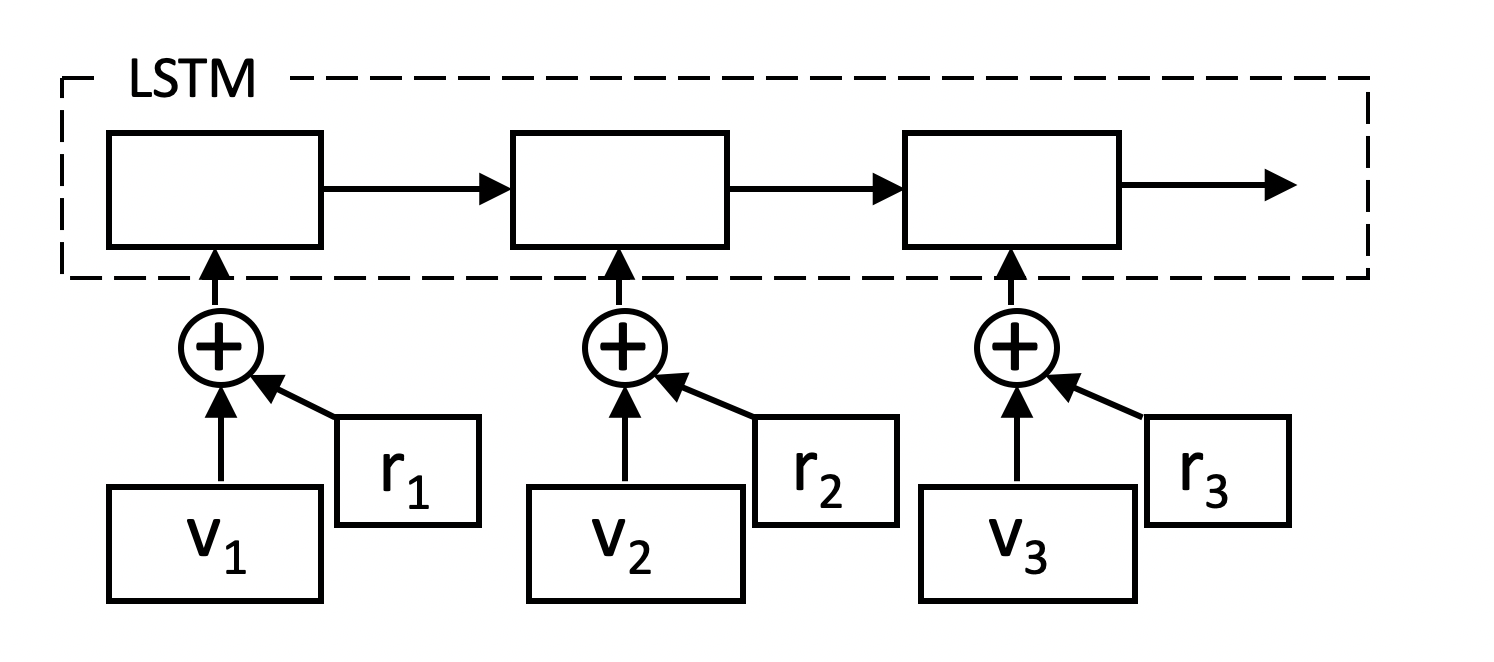
\includegraphics[width=0.55\linewidth]{AdvLSTM.png}
% 	\vspace{-0.8em}
	\caption{Adversarial LSTM with perturbed input}
	\label{fig:advLSTM}
	%\vspace{-1.4em}
\end{figure}

\section{(40 points) Adversarial Training as Proximal Mapping}

\begin{figure}[t]
% 	\vspace{-0.2em}
	\centering
	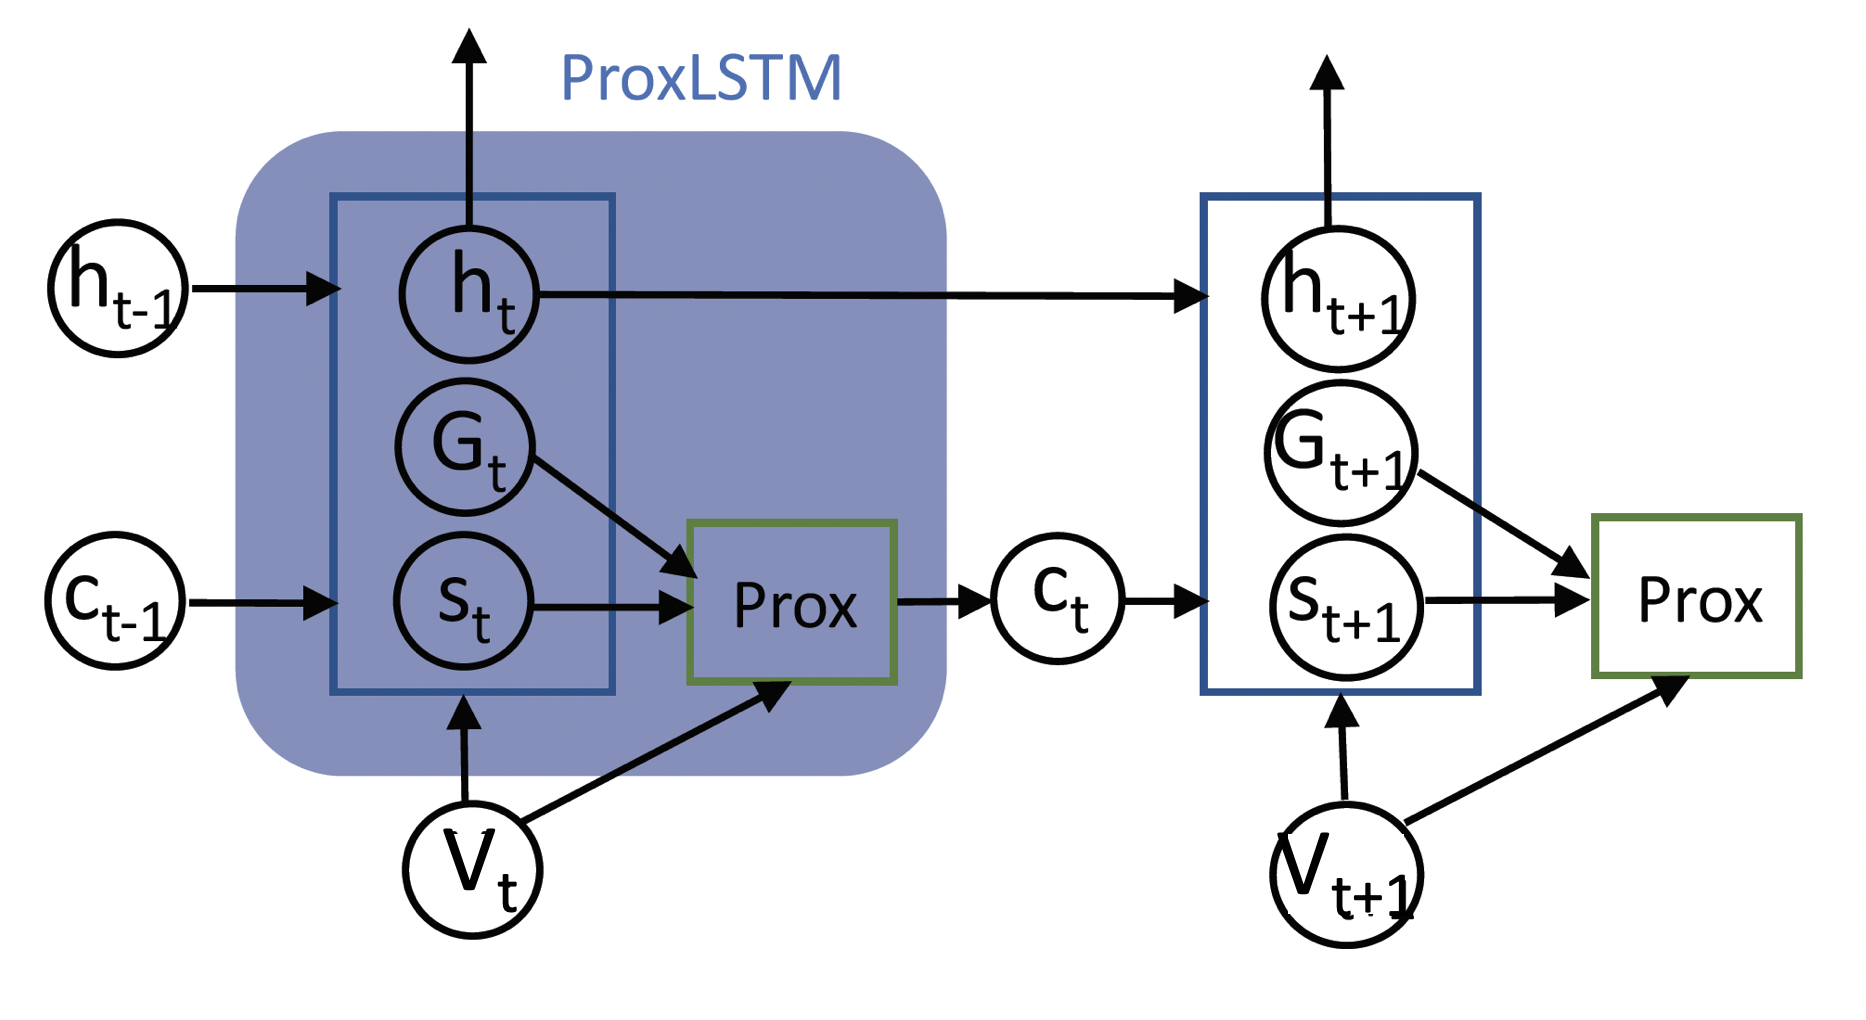
\includegraphics[width=0.5\linewidth]{ProxLSTM.png}
% 	\vspace{-2.0em}
	\caption{A proximal LSTM layer}
	\label{fig:proxLSTM}
	%\vspace{-1.4em}
\end{figure}

In this section, we will introduce a new adversarial training method that is based on proximal mapping. 
Let us recall the details of an LSTM cell.
At each time step, the evolution of the hidden state $c_t$ can be compactly represented by
$c_t = f(c_{t-1}, h_{t-1}, v_t)$,
while the output $h_t$ is updated by $h_t = g(c_{t-1}, h_{t-1}, v_t)$. 
We aim to encourage that the hidden state $c_t$ stays invariant, 
when each $v_t$ is perturbed by $r_t$ whose norm is bounded by some constant $\delta$.
To this end, we introduce an intermediate step 
$s_t = s_t(c_{t-1}, h_{t-1}, v_t)$ that computes the original hidden state,
and then the new hidden state $c_t$ is formed by moving $s_t$ towards the \emph{null} \emph{space} of the variation of $s_t$ under the perturbations on $v_t$,
while remaining close to $s_t$ by penalizing the Euclidean norm of $c_t - s_t$.
This leads to the following optimization (a.k.a. \textbf{proximal mapping}) that computes the new state $c_t$:

\vspace{-1.6em}
\begin{align}
\nonumber
c_t &:= \argmin_c {\smallfrac{\lambda}{2} \nbr{c - s_t}^2 
	+ \smallfrac{1}{2}\max_{r_t: \nbr{r_t} \le \delta} \inner{c}{\underbrace{s_t(c_{t-1}, h_{t-1}, v_t) - s_t(c_{t-1}, h_{t-1}, v_t + r_t)}_{\text{variation of } s_t \text{ under the perturbations on } v_t}}^2} \\
&\approx \argmin_c {\frac{\lambda}{2} \nbr{c - s_t}^2 
	+ \frac{1}{2} \max_{r_t: \nbr{r_t} \le \delta} \inner{c}{\frac{\partial}{\partial v_t} s_t(c_{t-1}, h_{t-1}, v_t) r_t}^2} \\
	\label{eq:proxmap}
&= \argmin_c {\smallfrac{\lambda}{2} \nbr{c - s_t}^2 
+ \smallfrac{\delta^2}{2}\nbr{c^\top G_t}^2}, 
\where G_t := \smallfrac{\partial}{\partial v_t} s_t(c_{t-1}, h_{t-1}, v_t),
\end{align}
The diagram is shown in Figure \ref{fig:proxLSTM}. 
By taking derivative of the objective in \eqref{eq:proxmap} with respect to $c$,
we obtain a closed-form solution for $c_t$: 
\begin{equation}
\label{eq:ct_expr}
    c_t = (I + \lambda^{-1} \delta^2 G_t G_t^\top)^{-1} s_t.
\end{equation} 

\begin{itemize}
    \item[a] \textbf{(30 points)} 
    Implement the ProxLSTMCell in \texttt{ProxLSTM.py} as shown in the blue area of Figure \ref{fig:proxLSTM}. 
    You need to implement both the \texttt{forward} and \texttt{backward} pass. Your implementation should use the built-in LSTMCell as a blackbox, 
    especially in computing the directional second-order derivative in \eqref{eq:ell_G_y} and \eqref{eq:ell_G_c}. 
    You can follow above formulations to implement the \texttt{forward} pass. 
    The \texttt{backward} pass contains second-order derivative, 
    and you may follow the computation details in Appendix \ref{app:gradient}.
    %
    \item[b] \textbf{(10 points)} Write a branch in \texttt{LSTMClassifier} so that it can handle \texttt{mode} = `ProxLSTM', you actually only need to change the original LSTMCell (for the `plain' mode) into the ProxLSTMCell you have implemented. 
    You should have already loaded the previously trained basic model to `Prox\_model' (Section \ref{sec:saveload}).
    
    Run the `Training Prox\_model' segment in \texttt{training.py} to see how it works. 
    According to \eqref{eq:ct_expr},
    $\lambda$ and $\delta$ make a difference only through the value of $\lambda^{-1} \delta^2$.
    So let us denote $\epsilon = \lambda^{-1} \delta^2$. 
    Tune $\epsilon$ to the best performance, 
    and then draw a figure whose x-axis is the training epoch, 
    and the y-axis is the test accuracy. 
    In the same figure, draw another three curves with $\epsilon = {0.1, 1.0, 5.0}$.
    The first curve (for the best $\epsilon$) can take as many epochs as you like, 
    but limit the training epoch to 100 for the other three curves.
    
    How does the performance change with respect to $\epsilon$?
    As for the other hyperparameters,
    you only need to pay a reasonable amount of effort in tuning them, 
    so that the performance is reasonably good.
    There is no need to find their optimal values.
\end{itemize}


\section {(10 points) Dropout and Batch Normalization}
\begin{itemize}
    \item[a] \textbf{(5 points)} 
    Try to add a dropout layer to the model, 
    and then train `Prox\_model' again. 
    Where did you add this layer (before convolution layer, after ProxLSTM layer, etc.) and how does it change the performance (improved, not helping, etc.)?
    %
    \item[b] \textbf{(5 points)} 
    Try to add batch normalization layer to the model, 
    and then train `Prox\_model' again. 
    Where did you add this layer (before convolution layer, after ProxLSTM layer, etc.) and how does it change the performance (improved, not helping, etc.)?
\end{itemize}

\appendix
\begin{center}
	\Huge \textbf{Appendix}
\end{center}
\label{sec:appdx}
\section{Backpropagation for ProxLSTM}

\label{app:gradient}
To concentrate on backpropagation,
we denote loss as $L$ and it only depends on the output of the last time step $T$, \ie, $h_T$.
From the final layer, we get $\frac{\partial L}{\partial h_T}$.
Then we can get $\frac{\partial L}{\partial h_{T-1}}$ and 
$\frac{\partial L}{\partial c_{T-1}}$ as in the standard LSTM ($G_T$ in the final layer can be ignored and 
$\frac{\partial L}{\partial c_T} = 0$). 
In order to compute the derivatives with respect to the weights $W$ in the LSTMs, we need to recursively compute 
$\frac{\partial L}{\partial h_{t-1}}$ and 
$\frac{\partial L}{\partial c_{t-1}}$,
given $\frac{\partial L}{\partial h_{t}}$ and 
$\frac{\partial L}{\partial c_{t}}$.
Once they are available, then
\begin{align}
\frac{\partial L}{\partial W} 
= \sum_{t=1}^T \cbr{\underbrace{\frac{\partial L}{\partial h_t}}_{\text{by } \eqref{eq:rec_ell_y}} 
	\underbrace{\frac{\partial}{\partial W} h_t(c_{t-1}, h_{t-1}, x_t)}_{\text{standard LSTM}}
	+ \underbrace{\frac{\partial L}{\partial c_t}}_{\text{by } \eqref{eq:rec_ell_c}} \underbrace{\frac{\partial}{\partial W} c_t(c_{t-1}, h_{t-1}, x_t)}_{\text{standard LSTM}}},
\end{align}
where the two $\frac{\partial}{\partial W}$ on the right-hand side are identical to the standard operations in LSTMs.
Here we use the Jacobian matrix arrangement for partial derivatives,
\ie,
if $f$ maps from $\RR^n$ to $\RR^m$,
then $\frac{\partial f(x)}{\partial x} \in \RR^{m \times n}$. 

Given $\frac{\partial L}{\partial c_{t}}$, we can first compute 
$\frac{\partial L}{\partial s_t}$ and $\frac{\partial L}{\partial G_t}$ based on the proximal map,
and the details will be provided in Section \ref{sec:grad_prox}.
Given their values,
we now compute
$\frac{\partial L}{\partial h_{t-1}}$ and 
$\frac{\partial L}{\partial c_{t-1}}$.
Firstly,
%
\begin{align}
\label{eq:rec_ell_y}
\frac{\partial L}{\partial h_{t-1}} = 
\underbrace{\frac{\partial L}{\partial h_t}}_{\text{by recursion}}
\underbrace{\frac{\partial h_t}{\partial h_{t-1}}}_{\text{std LSTM}}
+ \underbrace{\frac{\partial L}{\partial G_t} \frac{\partial G_t}{\partial h_{t-1}}}_{\text{by }\eqref{eq:ell_G_y}}
+ \underbrace{\frac{\partial L}{\partial s_t}}_{\text{by } \eqref{eq:ell_s}}
\underbrace{\frac{\partial s_t}{\partial h_{t-1}}}_{\text{std LSTM}}.
\end{align}
The terms $\frac{\partial h_t}{\partial h_{t-1}}$ and $\frac{\partial s_t}{\partial h_{t-1}}$ are identical to the operations in the standard LSTM.
The only remaining term is in fact a directional second-order derivative,
where the direction $\frac{\partial L}{\partial G_t}$ can be computed from from \eqref{eq:ell_G}:
\begin{align}
\label{eq:ell_G_y}
\frac{\partial L}{\partial G_t} \frac{\partial G_t}{\partial h_{t-1}} =
\frac{\partial L}{\partial G_t} \frac{\partial^2 }{\partial x_t \partial h_{t-1}} s_t(c_{t-1}, h_{t-1}, x_t)
= \frac{\partial}{\partial h_{t-1}} \inner{\underbrace{\frac{\partial L}{\partial G_t}}_{\text{by } \eqref{eq:ell_G}}}{\frac{\partial}{\partial x_t} s_t(c_{t-1}, h_{t-1}, x_t)}.
\end{align}
Such computations are well supported in most deep learning packages, such as PyTorch.
Secondly, 
\begin{align}
\label{eq:rec_ell_c}
\frac{\partial L}{\partial c_{t-1}} = 
\underbrace{\frac{\partial L}{\partial h_t}}_{\text{by recursion}}
\underbrace{\frac{\partial h_t}{\partial c_{t-1}}}_{\text{std LSTM}}
+ \underbrace{\frac{\partial J}{\partial G_t} \frac{\partial G_t}{\partial c_{t-1}}}_{\text{by }\eqref{eq:ell_G_c}}
+ \underbrace{\frac{\partial L}{\partial s_t}}_{\text{by } \eqref{eq:ell_s}}
\underbrace{\frac{\partial s_t}{\partial c_{t-1}}}_{\text{std LSTM}}.
\end{align}
The terms $\frac{\partial h_t}{\partial c_{t-1}}$ and $\frac{\partial s_t}{\partial c_{t-1}}$ are identical to the operations in the standard LSTM.
The only remaining term is in fact a directional second-order derivative:
\begin{align}
\label{eq:ell_G_c}
\frac{\partial L}{\partial G_t} \frac{\partial G_t}{\partial c_{t-1}} =
\frac{\partial L}{\partial G_t} \frac{\partial^2 }{\partial x_t \partial c_{t-1}} s_t(c_{t-1}, h_{t-1}, x_t)
= \frac{\partial}{\partial c_{t-1}} \inner{\underbrace{\frac{\partial L}{\partial G_t}}_{\text{by } \eqref{eq:ell_G}}}{\frac{\partial}{\partial x_t} s_t(c_{t-1}, h_{t-1}, x_t)}.
\end{align}


\subsection{Gradient Derivation for the Proximal Map}
\label{sec:grad_prox}

We now compute the derivatives involved in the proximal operator,
namely $\frac{\partial L}{\partial s_t}$ and $\frac{\partial L}{\partial G_t}$.
For clarify, let us omit the step index $t$, 
set $\epsilon = \lambda^{-1} \delta^2 = 1$ without loss of generality, 
and denote
\begin{align}
L = f(c), \where c := c(G,s) := (I + G G^\top)^{-1} s.
\end{align}
We first compute $\partial L / \partial s$ which is easier.
\begin{align}
\Delta L &:= f(c(G, s+\Delta s)) - f(c(G,s)) 
= \grad f(c)^\top (c(G,s+\Delta s) - c(G,s)) + o(\nbr{\Delta s})\\
&= \grad f(c)^\top (I+GG^\top)^{-1} \Delta s + o(\nbr{\Delta s}).
\end{align}
Here $o(\nbr{\Delta s})$ is a term that diminishes (tends to 0) faster than $\nbr{\Delta s}$.
Therefore, 
\begin{align}
\label{eq:ell_s}
\frac{\partial L}{\partial s} = \grad f(c)^\top (I+GG^\top)^{-1}.
\end{align}
We now move on to $\partial L / \partial G$.
Notice
%
\begin{align}
\Delta L := f(c(G+\Delta G,s)) - f(c(G,s)) 
= \grad f(c)^\top (c(G+\Delta G,s) - c(G,s)) + o(\nbr{\Delta G}).
\end{align}
Since
\begin{align}
&c(G+\Delta G,s) = (I+(G+\Delta G)(G + \Delta G)^\top)^{-1} s \\
= &\sbr{(I+GG^\top)^{\half} \rbr{I + (I+GG^\top)^{-\half} (\Delta G G^\top + G \Delta G^\top) (I+GG^\top)^{-\half}}(I+GG^\top)^{\half}}^{-1} s \\
= &(I+GG^\top)^{-\half} \rbr{I - (I+GG^\top)^{-\half} (\Delta G G^\top + G \Delta G^\top) (I+GG^\top)^{-\half} + o(\nbr{\Delta G})}(I+GG^\top)^{-\half} s \\
= & c(G,s) - (I+GG^\top)^{-1} (\Delta G G^\top + G \Delta G^\top) (I+GG^\top)^{-1} s + o(\nbr{\Delta G}),
\end{align}
we can finally obtain
\begin{align}
\Delta L
&= -\grad f(c)^\top (I+GG^\top)^{-1} (\Delta G G^\top + G \Delta G^\top) (I+GG^\top)^{-1} s + o(\nbr{\Delta G}) \\
&= -\tr \rbr{\Delta G^\top (I+GG^\top)^{-1} \rbr{\grad f(c) s^\top + s \grad f(c)^\top} (I+GG^\top)^{-1} G} + o(\nbr{\Delta G}).
\end{align}
So in conclusion,
\begin{align}
\frac{\partial L}{\partial G} &= - (I+GG^\top)^{-1} \rbr{\grad f(c) s^\top + s \grad f(c)^\top} (I+GG^\top)^{-1} G \\
\label{eq:ell_G}	
&= -(a c^\top + c a^\top)G,
\where a = (I+GG^\top)^{-1}\grad f(c).
\end{align}



\bibliography{references} \bibliographystyle{plain}
%\section{Convolutional filters}




\end{document}
